\PassOptionsToPackage{unicode=true}{hyperref} % options for packages loaded elsewhere
\PassOptionsToPackage{hyphens}{url}
%
\documentclass[ignorenonframetext,]{beamer}
\usepackage{pgfpages}
\setbeamertemplate{caption}[numbered]
\setbeamertemplate{caption label separator}{: }
\setbeamercolor{caption name}{fg=normal text.fg}
\beamertemplatenavigationsymbolsempty
% Prevent slide breaks in the middle of a paragraph:
\widowpenalties 1 10000
\raggedbottom
\setbeamertemplate{part page}{
\centering
\begin{beamercolorbox}[sep=16pt,center]{part title}
  \usebeamerfont{part title}\insertpart\par
\end{beamercolorbox}
}
\setbeamertemplate{section page}{
\centering
\begin{beamercolorbox}[sep=12pt,center]{part title}
  \usebeamerfont{section title}\insertsection\par
\end{beamercolorbox}
}
\setbeamertemplate{subsection page}{
\centering
\begin{beamercolorbox}[sep=8pt,center]{part title}
  \usebeamerfont{subsection title}\insertsubsection\par
\end{beamercolorbox}
}
\AtBeginPart{
  \frame{\partpage}
}
\AtBeginSection{
  \ifbibliography
  \else
    \frame{\sectionpage}
  \fi
}
\AtBeginSubsection{
  \frame{\subsectionpage}
}
\usepackage{lmodern}
\usepackage{amssymb,amsmath}
\usepackage{ifxetex,ifluatex}
\usepackage{fixltx2e} % provides \textsubscript
\ifnum 0\ifxetex 1\fi\ifluatex 1\fi=0 % if pdftex
  \usepackage[T1]{fontenc}
  \usepackage[utf8]{inputenc}
  \usepackage{textcomp} % provides euro and other symbols
\else % if luatex or xelatex
  \usepackage{unicode-math}
  \defaultfontfeatures{Ligatures=TeX,Scale=MatchLowercase}
\fi
% use upquote if available, for straight quotes in verbatim environments
\IfFileExists{upquote.sty}{\usepackage{upquote}}{}
% use microtype if available
\IfFileExists{microtype.sty}{%
\usepackage[]{microtype}
\UseMicrotypeSet[protrusion]{basicmath} % disable protrusion for tt fonts
}{}
\IfFileExists{parskip.sty}{%
\usepackage{parskip}
}{% else
\setlength{\parindent}{0pt}
\setlength{\parskip}{6pt plus 2pt minus 1pt}
}
\usepackage{hyperref}
\hypersetup{
            pdftitle={CS5014 Machine Learning},
            pdfauthor={Lei Fang},
            pdfborder={0 0 0},
            breaklinks=true}
\urlstyle{same}  % don't use monospace font for urls
\newif\ifbibliography
\setlength{\emergencystretch}{3em}  % prevent overfull lines
\providecommand{\tightlist}{%
  \setlength{\itemsep}{0pt}\setlength{\parskip}{0pt}}
\setcounter{secnumdepth}{0}

% set default figure placement to htbp
\makeatletter
\def\fps@figure{htbp}
\makeatother

%\usepackage[latin1]{inputenc}

\usepackage{graphicx}
\usepackage{rotating}
%\setbeamertemplate{caption}[numbered]
\usepackage{hyperref}
\usepackage{caption}
\usepackage[normalem]{ulem}
%\mode<presentation>
\usepackage{wasysym}
\usepackage{amsmath}
\usepackage{mathtools}
\usepackage[skins,theorems]{tcolorbox}
\tcbset{highlight math style={enhanced,
  colframe=red,colback=white,arc=0pt,boxrule=1pt}}

\newcommand{\normal}[2]{\ensuremath{\mathcal{N}\left (#1,#2 \right )}}
\newcommand{\Gaussian}[3]{\ensuremath{\frac{1}{\sqrt{2\pi}#3}
\text{exp}\left \{-\frac{1}{2#3^2} (#1-#2)^2 \right \}}}
\newcommand{\argmax}{\operatornamewithlimits{argmax}}
\newcommand{\expo}[1]{\ensuremath{\text{exp}\left \{ #1 \right \}}}
\newcommand{\studentt}[4]{\ensuremath{\mathcal{T}_{#4}(#1,#2,#3)}}
\newcommand{\vv}[1]{\boldsymbol{#1}}
\newcommand{\Prb}{\ensuremath{\mathbb{P}}}
\newcommand{\studenttk}[4]{\ensuremath{\mathcal{T}_{#4}(#1,#2,#3)}}
\newcommand{\argmin}{\operatornamewithlimits{argmin}}
\newcommand{\NIG}{\mathcal{NIG}}
\newcommand{\N}{\mathcal{N}}
\newcommand{\T}{\mathcal{T}}
\newcommand{\IG}{\mathcal{IG}}
\newcommand{\IW}{\mathcal{IW}}
\newcommand{\NNIW}{\mathcal{NNIW}}
\newcommand{\vct}{\text{vec}}
\newcommand{\NN}{\mathcal{NN}}
\newcommand{\tr}{\text{tr}}



\newcommand{\E}[1]{\ensuremath{\mathbb{E}[#1]}}
\newcommand{\Var}[1]{\mathrm{Var}[#1]}
\newcommand{\Cov}[2]{\mathrm{Cov}[#1,#2]}
\newcommand{\Cor}[2]{\mathrm{Cor}[#1,#2]}


% \setbeamertemplate{navigation symbols}{}



%\titlegraphic{\includegraphics[width=0.3\paperwidth]{\string~/Dropbox/teaching/clemson-academic.png}}
\titlegraphic{
\includegraphics[width=0.12\paperwidth]{crest.pdf}}
\setbeamertemplate{title page}[empty]

\setbeamerfont{subtitle}{size=\small}

\setbeamercovered{transparent}

\definecolor{clemsonpurple}{HTML}{522D80}
\definecolor{stablue}{HTML}{0052cc}
\definecolor{stared}{HTML}{ff4d4d}
\definecolor{clemsonorange}{HTML}{F66733}

\setbeamercolor{frametitle}{fg=stablue,bg=white}
\setbeamercolor{title}{fg=stablue,bg=white}
\setbeamercolor{local structure}{fg=stablue}
\setbeamercolor{section in toc}{fg=stablue,bg=white}
\setbeamercolor{subsection in toc}{fg=stared,bg=white}
\setbeamercolor{item projected}{fg=stablue,bg=white}
\setbeamertemplate{itemize item}{\color{stablue}$\bullet$}
\setbeamertemplate{itemize subitem}{\color{stablue}\scriptsize{$\bullet$}}
\let\Tiny=\tiny

%\makeatletter
%\setbeamertemplate{footline}{%
%\leavevmode
%\vbox{\begin{beamercolorbox}[dp=1.25ex,ht=2.75ex]{fg=black}%
%  \hspace*{1em}\insertsectionhead%
%  \ifx\insertsubsectionhead\@empty\relax\else$\quad\mid\quad$\insertsubsectionhead\fi :
%  \end{beamercolorbox}%
%  }%
%}
%\makeatother

\setbeamercolor{footercl}{fg=white,bg=stablue}
\setbeamerfont{stafont}{size = \large}
\setbeamerfont{footerfont}{size = \tiny}
% \makeatother
% \setbeamertemplate{footline}
% {
%   \leavevmode%
%   \hbox{%
%   \begin{beamercolorbox}[wd=.5\paperwidth,ht=5ex,dp=1ex, left]{footercl}%
%     \usebeamerfont*{stafont}\hspace*{1ex}\insertshortinstitute
%   \end{beamercolorbox}%
%   \begin{beamercolorbox}[wd=.25\paperwidth,ht=5ex,dp=1ex,center]{footercl}%
%     \usebeamerfont*{footerfont}\insertshorttitle\hspace*{1ex} \insertframenumber{}
%   \end{beamercolorbox}%
%   \begin{beamercolorbox}[wd=.25\paperwidth,ht=5ex,dp=1ex,right]{footercl}%
%    
\includegraphics[height=5ex]{stalogo.png}
%   \end{beamercolorbox}}%
%   \vskip0pt%
% }
% \makeatletter
\makeatletter
\setbeamertemplate{footline}
{
  \leavevmode%
  \hbox{%
  \fontsize{13}{13}\fontfamily{ppl}\selectfont
  \begin{beamercolorbox}[wd=.5\paperwidth,ht=2.25ex,dp=1ex,left]{footercl}%
    \usebeamerfont{author in head/foot}\hspace*{1ex}\insertshortinstitute
   \end{beamercolorbox}%
   \begin{beamercolorbox}[wd=.25\paperwidth,ht=2.25ex,dp=1ex,right]{footercl}%
    % \hfill\hfill\hfill\hfill\hfill\hfill\hfill\hfill\hfill\hfill
    \parbox{.25\paperwidth}{\fontfamily{cmss}\selectfont{\hfill\hfill \usebeamerfont{footerfont}\insertshorttitle~\insertframenumber{}}}
  \end{beamercolorbox}%
  \begin{beamercolorbox}[wd=.25\paperwidth,ht=2.25ex,dp=1ex,left]{footercl}%
    \parbox{.25\paperwidth}{\hfill
\includegraphics[height=1cm]{stalogo.png}}% original: 2ex
  \end{beamercolorbox}}%
  \vskip0pt%
}
\makeatother

\setbeamertemplate{navigation symbols}{}

% \AtBeginDocument{\author[L. Fang]{Lei Fang} \institute[www.st-andrews.ac.uk]{School of Computer Science, University of St Andrews}}

% \newcommand{\Ffootline}{%                   %%defines a new command called \Ffootline
% %\insertshortauthor,                         %%puts the abbreviated form of the author's name in the left corner
% \insertshorttitle,
% \insertshortinstitute, 
% \insertshortdate %%puts the abbreviated form of the author's institution in the middle
% \hfill
% \insertsection,
% \insertframenumber/\inserttotalframenumber} %%includes the current slide number over the total slide number in the right corner
% \setbeamertemplate{footline}{%              %%sets the options for the footline
% \usebeamerfont{structure}                   %%uses the same fonts adopted for the structure of the presentation 
% \Tiny\hspace*{4mm} \Ffootline \hspace{4mm}  %%sets the size of the font to Tiny and includes the content of the \Ffootline
% }                                           %%command leaving a margin of 4mm to the right and left of the content.



\AtBeginPart{}
\AtBeginSection{}
\AtBeginSubsection{}
\AtBeginSubsubsection{}
\setlength{\emergencystretch}{0em}
\setlength{\parskip}{0pt}
\AtBeginDocument{\author[L. Fang]{Lei Fang} \title[L2 Maths Review]{CS5014 Machine Learning}\institute[www.st-andrews.ac.uk]{School of Computer Science, University of St Andrews}}

\title{CS5014 Machine Learning}
\providecommand{\subtitle}[1]{}
\subtitle{Lecture 2 Maths background review}
\author{Lei Fang}
\date{Spring 2021}

\begin{document}
\frame{\titlepage}

\hypertarget{introduction}{%
\section{Introduction}\label{introduction}}

\begin{frame}{So why this review session ?}
\protect\hypertarget{so-why-this-review-session}{}

Maths is useful

\begin{itemize}
\tightlist
\item
  rigorous and concise way of communicating results
\item
  help us understand why \emph{and} why not models work
\item
  be able to derive your own model and algorithms!
\end{itemize}

\pause 
\bigskip

Refresher on essential concepts

\begin{itemize}
\tightlist
\item
  only a refresher; we expect you have learnt them

  \begin{itemize}
  \tightlist
  \item
    don't expect to know everything after this
  \end{itemize}
\item
  not complete and not rigorous
\end{itemize}

\pause

\bigskip A chance for self-assessment

\begin{itemize}
\tightlist
\item
  identify rusty area
\item
  do self studies afterwards
\item
  maths learning should be never-ending :-)
\end{itemize}

\end{frame}

\begin{frame}{Mathematics for machine learning}
\protect\hypertarget{mathematics-for-machine-learning}{}

Linear algebra

\begin{itemize}
\tightlist
\item
  leap forward from 1-d to \(N\)-dimensional
\item
  number line axis to a plane and hyper-space 
\end{itemize}

\bigskip Calculus

\begin{itemize}
\tightlist
\item
  continuous (real-valued) functions by approximation, (say
  \emph{polynomial})

  \begin{itemize}
  \tightlist
  \item
    \(y= sin(x)\) is approximated by \(y=x\) when \(x \approx 0\)
  \end{itemize}
\item
  useful for optimisation
\end{itemize}

\bigskip Probability theory and statistics

\begin{itemize}
\tightlist
\item
  study of uncertainty: uncertainty is the norm

  \begin{itemize}
  \tightlist
  \item
    e.g.~rain tomorrow? blood pressure measurement (reading error)?
  \end{itemize}
\item
  how to generalise your results

  \begin{itemize}
  \tightlist
  \item
    from one sample to the universe: training error \(\rightarrow\)
    testing?
  \end{itemize}
\end{itemize}

\end{frame}

\begin{frame}{Useful textbook and references (read the italic entries!)}
\protect\hypertarget{useful-textbook-and-references-read-the-italic-entries}{}

\textbf{Linear algebra}

\begin{itemize}
\tightlist
\item
  \href{https://api.semanticscholar.org/CorpusID:18857001}{\emph{Learning
  from Data Supplementary Mathematics (Vector and Linear Algebra) by
  David Barber}; https://api.semanticscholar.org/CorpusID:18857001}
\item
  \href{https://www.deeplearningbook.org/contents/linear_algebra.html}{\emph{Chapter
  2 of Deep Learning by Ian Goodfellow, Yoshua Bengio and Aaron
  Courville}
  https://www.deeplearningbook.org/contents/linear\_algebra.html}
\item
  \href{http://math.mit.edu/~gs/linearalgebra/}{Introduction to Linear
  Algebra by Gilbert Strang;
  http://math.mit.edu/\textasciitilde{}gs/linearalgebra/}
\item
  \href{https://www2.imm.dtu.dk/pubdb/pubs/3274-full.html}{The Matrix
  Cookbook by Kaare Brandt Petersen, Michael Syskind Pedersen;
  https://www2.imm.dtu.dk/pubdb/pubs/3274-full.html}

  \begin{itemize}
  \tightlist
  \item
    useful as a reference manual
  \end{itemize}
\end{itemize}

\end{frame}

\begin{frame}{}
\protect\hypertarget{section}{}

\textbf{Probability theory}

\begin{itemize}
\tightlist
\item
  \href{http://www.inference.org.uk/itprnn/book.pdf}{\emph{Chapter
  2.1-2.3 Information Theory, Inference, and Learning Algorithms by
  David J.C. MacKay} http://www.inference.org.uk/itprnn/book.pdf}
\item
  \href{https://www.deeplearningbook.org/contents/prob.html}{\emph{Chapter
  3.1-3.9 of Deep Learning by Ian Goodfellow, Yoshua Bengio and Aaron
  Courville} https://www.deeplearningbook.org/contents/prob.html}
\item
  Introduction to Probability Models by Sheldon Ross

  \begin{itemize}
  \tightlist
  \item
    chapter 1; chapter 2.1-2.5, 2.8; chapter 3.1-3.5
  \end{itemize}
\end{itemize}

\textbf{Calculus}

\begin{itemize}
\tightlist
\item
  Use your book of choice; read multivariate calculus part as well
\item
  \href{http://web4.cs.ucl.ac.uk/staff/D.Barber/textbook/200620.pdf}{Appendix
  of Bayesian Reasoning and Machine Learning by David Barber
  http://web4.cs.ucl.ac.uk/staff/D.Barber/textbook/200620.pdf}
\end{itemize}

\end{frame}

\hypertarget{linear-algebra}{%
\section{Linear Algebra}\label{linear-algebra}}

\begin{frame}{Linear algebra: basic concepts}
\protect\hypertarget{linear-algebra-basic-concepts}{}

\begin{itemize}
\tightlist
\item
  vectors \bigskip
\item
  norms and projection \bigskip
\item
  linear independence, span, subspace \bigskip
\item
  matrices, linear transformation \bigskip
\item
  rank, determinant, trace
\end{itemize}

\end{frame}

\begin{frame}{Vector}
\protect\hypertarget{vector}{}

A vector is a collection of \(n\) salars

\begin{itemize}
\tightlist
\item
  \(\vv{a} \in R^n\), default option is column vector i.e. \(n\times 1\)
\item
  represents a \textbf{displacement} in \(R^n\)
\item
  e.g.
  \(\vv{a} = \begin{bmatrix}  2 \\  1  \end{bmatrix}, \textcolor{red}{\vv{b} = \begin{bmatrix}  1 \\  2  \end{bmatrix}}\)
  (or \(\vv{a} = [2, 1]^T\) to save space) \bigskip   
\end{itemize}

\begin{center}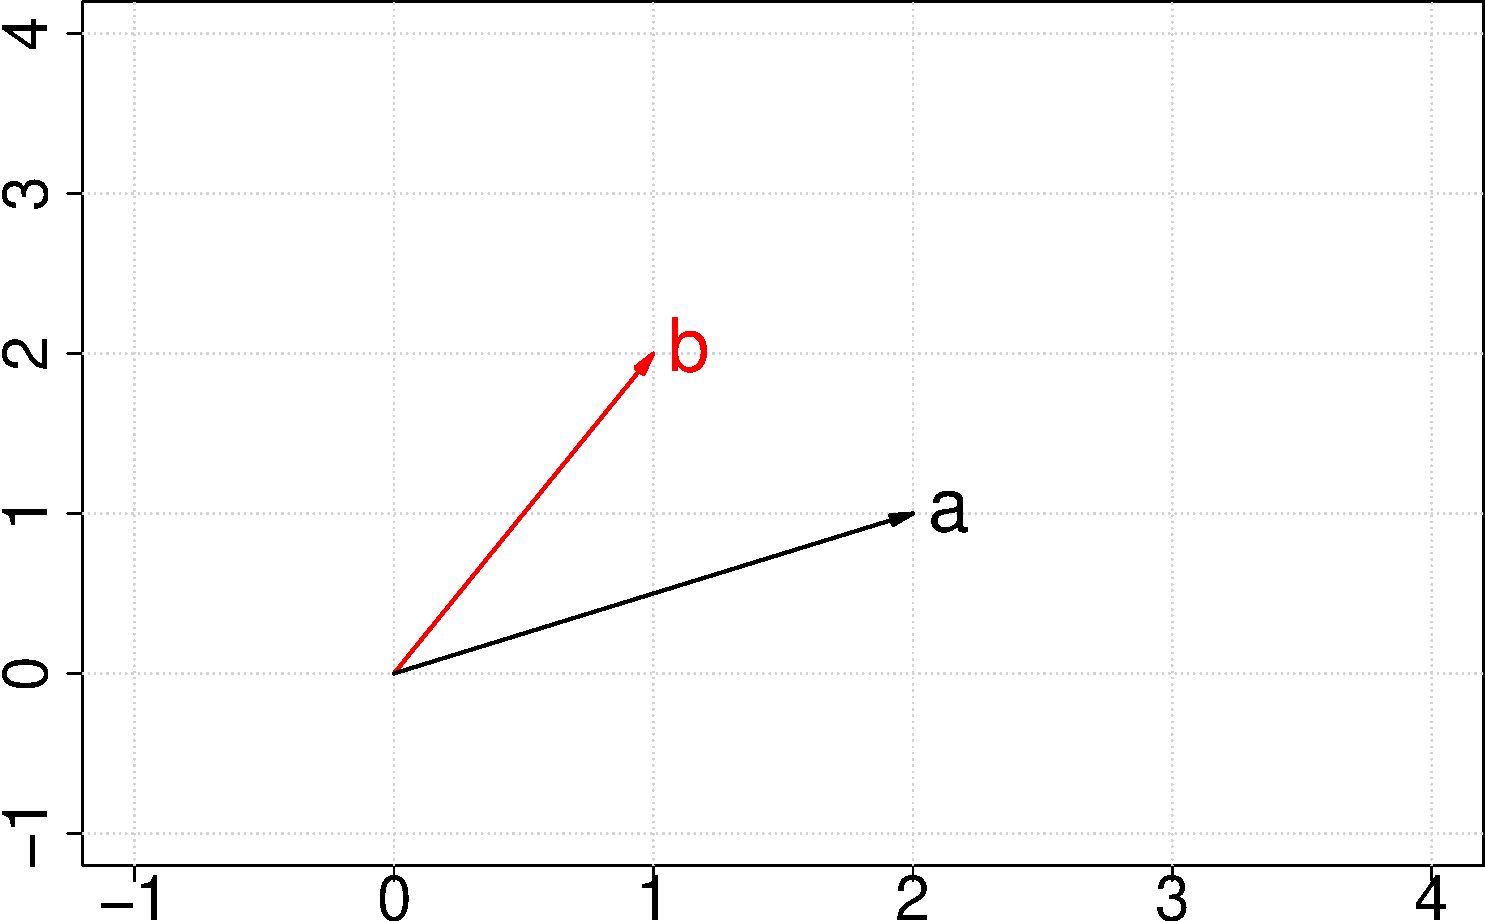
\includegraphics[width=0.49\linewidth]{math4ml_files/figure-beamer/figures-side-1} \end{center}

\end{frame}

\begin{frame}{}
\protect\hypertarget{section-1}{}

\bigskip

Some 3-d vectors
\(\vv{c} = \begin{bmatrix}  2 \\  2 \\  2  \end{bmatrix}, \vv{d} = \begin{bmatrix}  2 \\  0 \\  0  \end{bmatrix}, \vv{e} = \begin{bmatrix}  3 \\  2 \\  1  \end{bmatrix}\)
\bigskip   

\begin{center}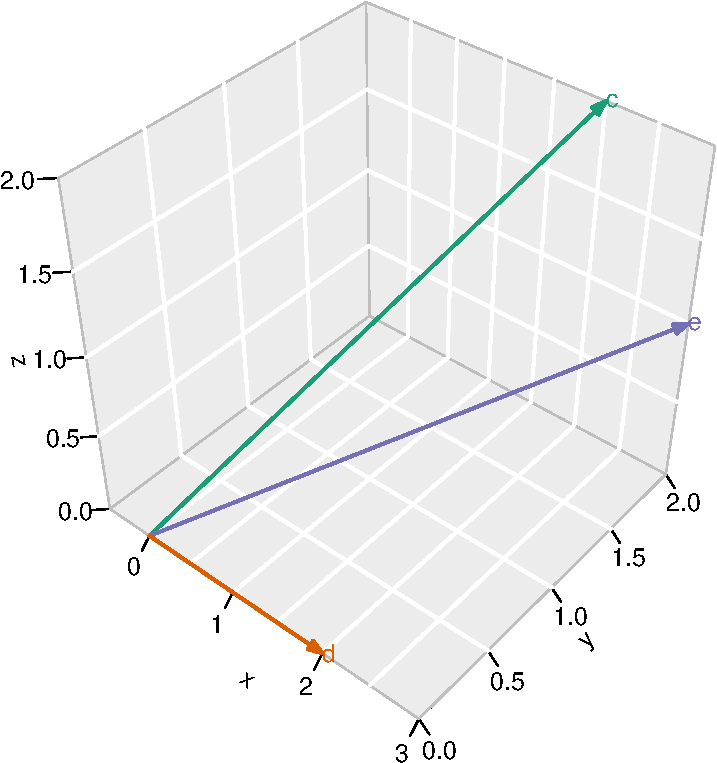
\includegraphics[width=0.55\linewidth]{math4ml_files/figure-beamer/unnamed-chunk-2-1} \end{center}

\end{frame}

\begin{frame}{Vector addition}
\protect\hypertarget{vector-addition}{}

\[\vv{a}+\vv{b} = \begin{bmatrix}
           a_1 \\
           a_2 \\
           \vdots\\
           a_d
         \end{bmatrix} +  \begin{bmatrix}
           b_1 \\
           b_2 \\
           \vdots\\
           b_d
         \end{bmatrix} = \begin{bmatrix}
           a_1+b_1 \\
           a_2+b_2 \\
           \vdots\\
           a_d+b_d
         \end{bmatrix}\]

\begin{itemize}
\tightlist
\item
  generalisation from scalar addition; remember 2+1 on a number axis ?
\item
  parallelogram rule \bigskip
\end{itemize}

\begin{center}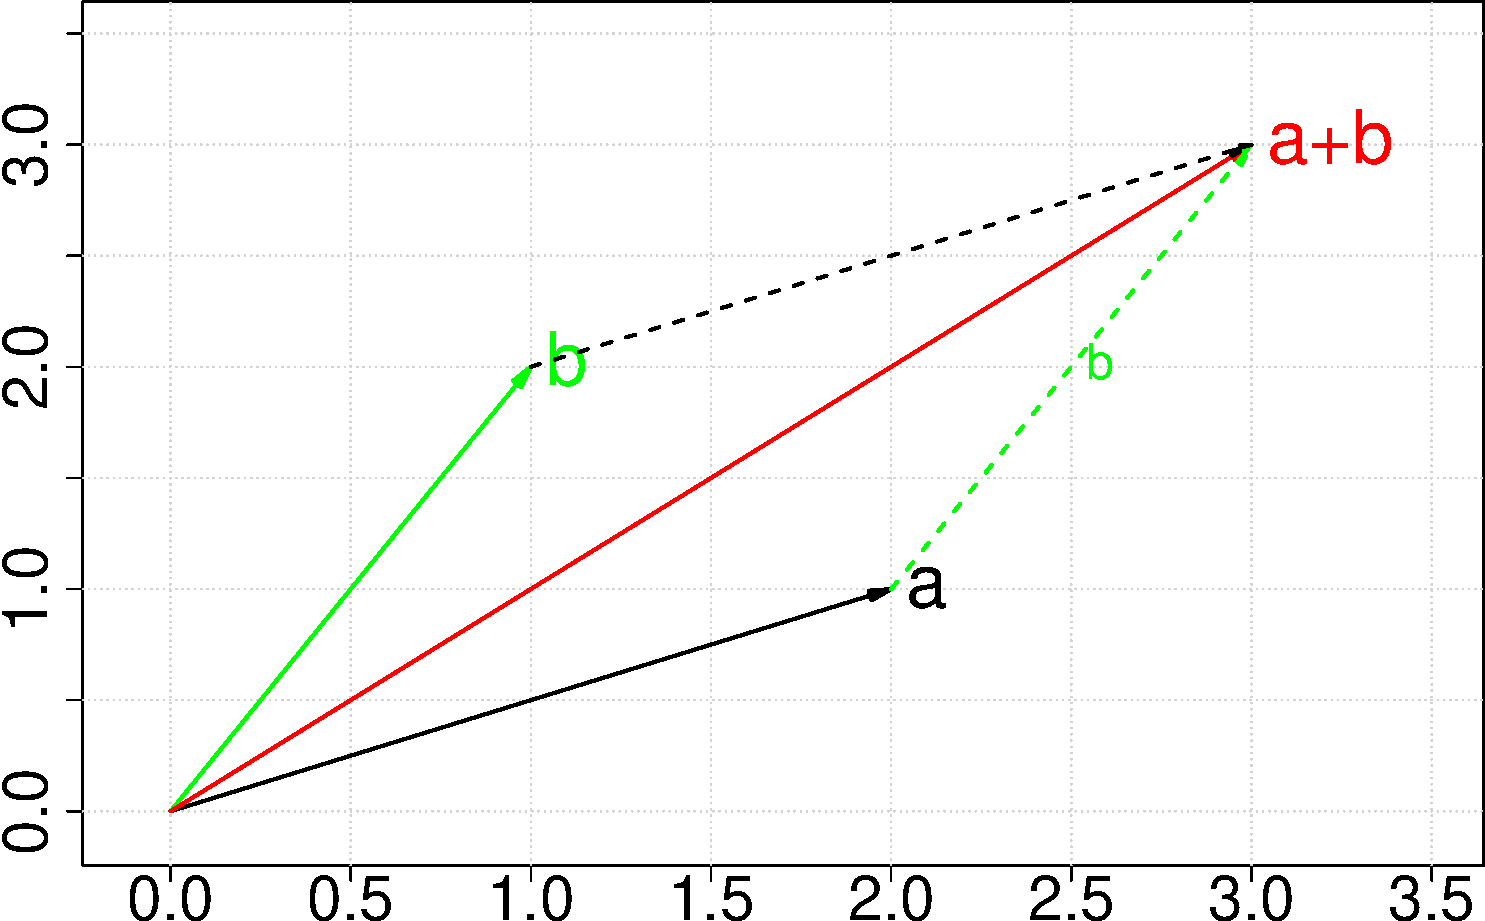
\includegraphics[width=0.5\linewidth]{math4ml_files/figure-beamer/unnamed-chunk-3-1} \end{center}

\end{frame}

\begin{frame}{Vector scaling/multiplication}
\protect\hypertarget{vector-scalingmultiplication}{}

\[k\cdot \vv{a} = k \cdot \begin{bmatrix}
           a_1 \\
           a_2 \\
           \vdots\\
           a_d
         \end{bmatrix} = \begin{bmatrix}
           k\times a_1 \\
           k\times a_2 \\
           \vdots\\
           k\times a_d
         \end{bmatrix}, k\in R \text{ or a scalar}\]

\begin{itemize}
\tightlist
\item
  geometrically, scaling means shrinking or streching a vector

  \begin{itemize}
  \tightlist
  \item
    the direction does not change but length changes
  \end{itemize}
\item
  arithmetically,
  \(n\cdot \vv{a} = \vv{a}+\ldots+ \vv{a}=\sum_n \vv{a}\)
\item
  \(0\cdot \vv{a} = \vv{0}\)
\end{itemize}

\begin{center}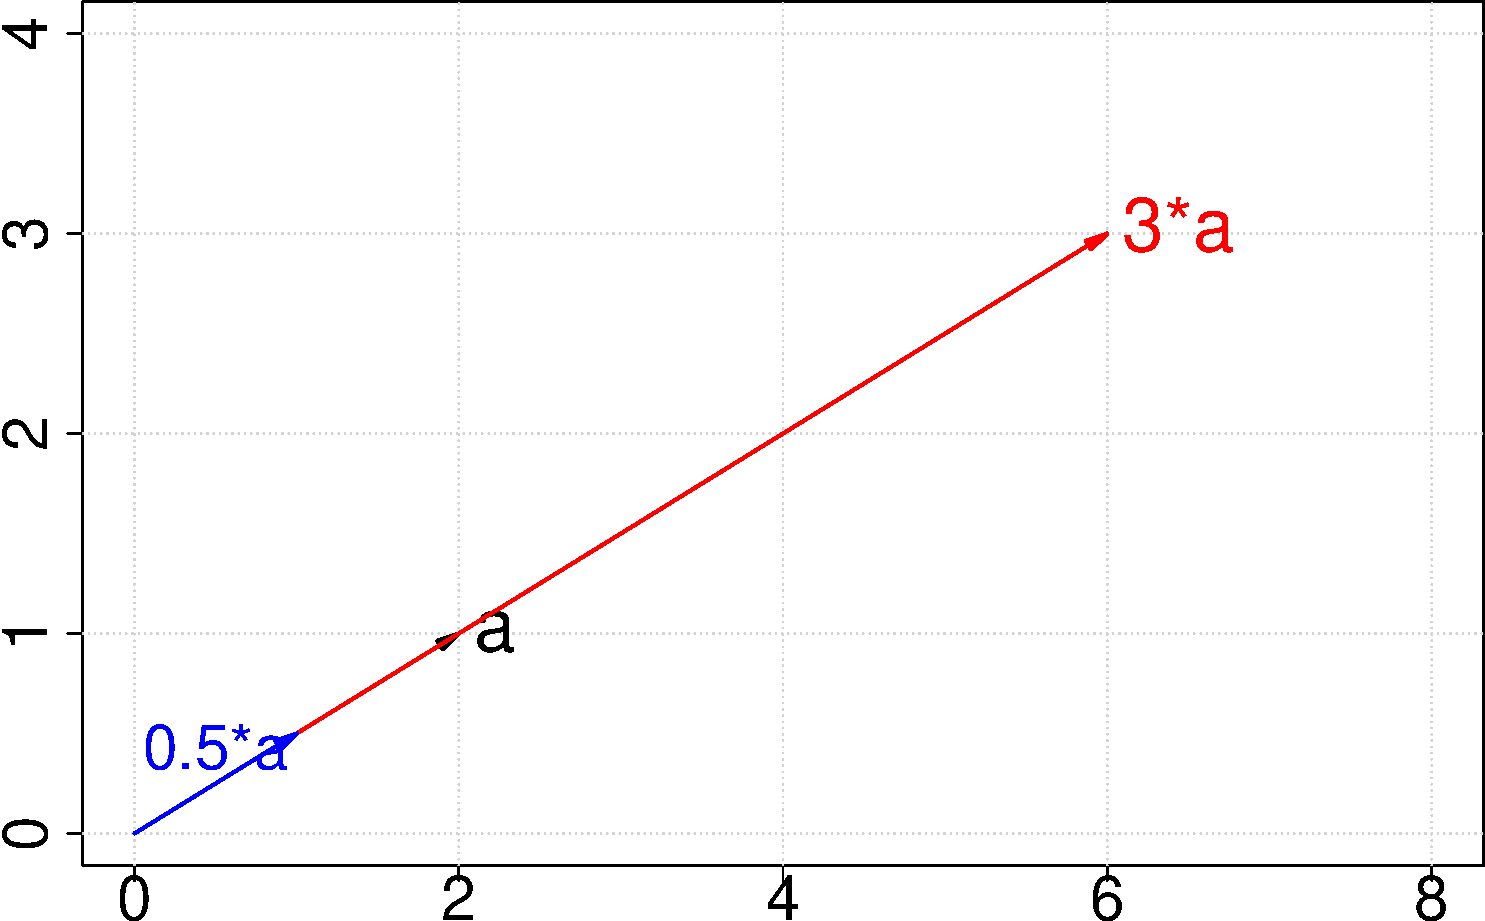
\includegraphics[width=0.45\linewidth]{math4ml_files/figure-beamer/unnamed-chunk-4-1} \end{center}

\end{frame}

\begin{frame}{Inner product}
\protect\hypertarget{inner-product}{}

\[\vv{a}^T \vv{b} = [a_1, a_2\ldots, a_d] \cdot \begin{bmatrix}
            b_1 \\
            b_2 \\
           \vdots\\
            b_d
         \end{bmatrix} = \sum_{i=1}^d a_i\times b_i\]

\begin{itemize}
\tightlist
\item
  \(\vv{a}^T \vv{b} = \vv{b}^T\vv{a}\) and the result is a scalar
\item
  \(\vv{a}^T(\vv{b}+\vv{c}) = \vv{a}^T\vv{b}+ \vv{a}^T\vv{c}\)
\item
  \((k\vv{a})^T\vv{b} = \vv{a}^T(k\vv{b})= k(\vv{a}^T\vv{b})\)
\item
  \(\vv{a}^T \vv{a} = \sum_{i=1}^d a_i^2\) is squared Euclidean distance
  between \(\vv{a}\) and \(\vv{0}\)
\item
  \(\vv{a}^T \vv{a} \geq 0\) and \(\vv{a}=\vv{0}\) if and only if
  \(\vv{a}^T\vv{a} =0\)
\end{itemize}

\end{frame}

\begin{frame}{Inner product and projection}
\protect\hypertarget{inner-product-and-projection}{}

Another interpretation:
\[\vv{a}^T \vv{b} = \|\vv{a}\| \|\vv{b}\|cos \theta\]

\begin{center}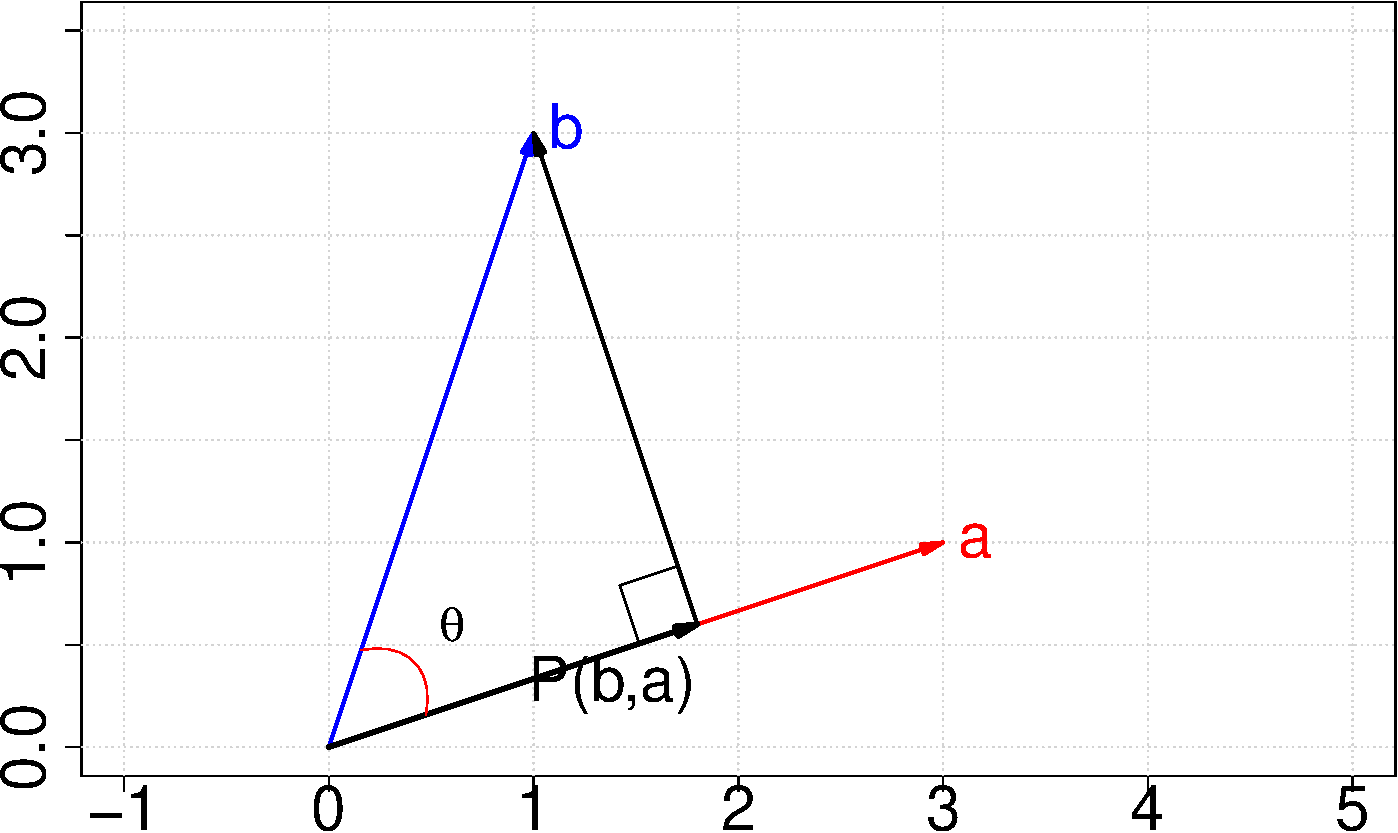
\includegraphics[width=0.45\linewidth]{math4ml_files/figure-beamer/unnamed-chunk-5-1} \end{center}

\begin{itemize}
\tightlist
\item
  \(\theta\) is the angle between \(\vv{a}, \vv{b}\)

  \begin{itemize}
  \tightlist
  \item
    \(\vv{a}^T\vv{b}=0\) if and only if \(\vv{a} \perp \vv{b}\) 
  \end{itemize}
\item
  \(\|\vv{b}\|cos \theta = \|P(\vv{b}, \vv{a})\|\) is the projected
  length of \(\vv{b}\) on \(\vv{a}\)
\item
  \(P(\vv{b}, \vv{a})\) denotes the projected vector of \(\vv{b}\) to
  \(\vv{a}\)
  \[P(\vv{b}, \vv{a}) = \|\vv{b}\|cos \theta * \frac{\vv{a}}{\|\vv{a}\|} =  \frac{\vv{a}^T\vv{b}}{\vv{a}^T\vv{a}}  \vv{a}\]
\end{itemize}

\end{frame}

\begin{frame}{Matrix}
\protect\hypertarget{matrix}{}

A rectangular array of real numbers \(A\in R^{m\times n}\)
\[\vv{A} = \begin{bmatrix}
a_{11} & a_{12} & \ldots & a_{1n}\\
a_{21} & a_{22} & \ldots & a_{2n} \\
\vdots & \vdots & & \vdots \\
a_{m1} & a_{m2} & \ldots & a_{mn}
\end{bmatrix}  = \begin{bmatrix}
\vert & \vert &  & \vert\\
\vv{a}_1 & \vv{a}_2 & \ldots & \vv{a}_{n} \\
\vert & \vert & & \vert 
\end{bmatrix} = \begin{bmatrix}
\text{---} & \vv{\tilde{a}}_1 & \text{---}\\
\vdots & \vdots & \vdots  \\
\text{---} & \vv{\tilde{a}}_m & \text{---}
\end{bmatrix} \]

\begin{itemize}
\tightlist
\item
  can be viewed as a collection of n column vectors
  \(\vv{A} = [\vv{a}_1, \vv{a}_2, \ldots, \vv{a}_n]\);
\item
  or row vectors
  \(\vv{A} = [\vv{\tilde{a}}_1^T, \vv{\tilde{a}}_2^T, \ldots, \vv{\tilde{a}}_m^T]^T\)
\item
  sometimes written as \(\vv{A} = (a_{ij})\)
  \(i= 1,\ldots m, j= 1,\ldots, n\)
\end{itemize}

\end{frame}

\begin{frame}{Matrix operations}
\protect\hypertarget{matrix-operations}{}

\begin{itemize}
\tightlist
\item
  addition: \(\vv{A} +\vv{B} =\vv{C}=(c_{ij})\) where
  \(c_{ij} = a_{ij} +b_{ij}\)
\item
  scaling: \(k\vv{A}= \vv{C}\) where \(c_{ij} =k* a_{ij}\)
\item
  transpose: \(\vv{A}^T = \vv{C}\) where \(c_{ij} = a_{ji}\)
\item
  multiplication: Let
  \(\vv{A}\in R^{m\times s}, \vv{B} \in R^{s\times n}\)
  \[\vv{AB} = \vv{C}, \vv{C} \in R^{m\times n}\] where
  \[c_{ij} = \sum_{k=1}^s a_{ik}b_{jk}\] or
  \(c_{ij} = \vv{\tilde{a}}_i^T\vv{b}_j\)

  \begin{itemize}
  \tightlist
  \item
    \(\vv{A}(\vv{BC}) =(\vv{AB})\vv{C}\)
  \item
    \(\vv{AB} \neq \vv{BA}\)
  \item
    \((\vv{AB})^T = \vv{B}^T \vv{A}^T\)
  \item
    \(\vv{I}\) identity matrix: \(\vv{I}\vv{A} = \vv{A}\) or
    \(\vv{AI}=\vv{A}\)
  \end{itemize}
\item
  inverse (only square matrix):
  \(\vv{A}^{-1} \vv{A}= \vv{AA}^{-1} =\vv{I}\)
\end{itemize}

\end{frame}

\begin{frame}{Examples}
\protect\hypertarget{examples}{}

\[
\begin{bmatrix}2&3 \\6&4 \\1&1 \\\end{bmatrix} + \begin{bmatrix}5&2&2 \\1&1&2 \\\end{bmatrix}  = ?
\] \pause it is not allowed as the dimensions do not match

\[
\begin{bmatrix}2&3 \\6&4 \\1&1 \\\end{bmatrix}^T   = \begin{bmatrix}2&6&1 \\3&4&1 \\\end{bmatrix}
\]

\end{frame}

\begin{frame}{Example}
\protect\hypertarget{example}{}

\[
\begin{bmatrix}2&3 \\6&4 \\1&1 \\\end{bmatrix} \times \begin{bmatrix}5&2&2 \\1&1&2 \\\end{bmatrix}  =  \begin{bmatrix} \tcbhighmath[boxrule=2pt,arc=1pt,colback=blue!10!white,colframe=blue,
  drop fuzzy shadow=red]{ 2\times 5+3\times 1 }& c_{12} & c_{13}\\
c_{21}& c_{22} & c_{23}\\
c_{31}& c_{32} & c_{33}
\end{bmatrix}
\] \[
\begin{bmatrix}2&3 \\6&4 \\1&1 \\\end{bmatrix} \times \begin{bmatrix}5&2&2 \\1&1&2 \\\end{bmatrix}  =  \begin{bmatrix}13&7&10 \\34&16&20 \\6&3&4 \\\end{bmatrix}
\]

\[
\begin{bmatrix}5&2&2 \\1&1&2 \\\end{bmatrix} \times \begin{bmatrix}2&3 \\6&4 \\1&1 \\\end{bmatrix}  =  \begin{bmatrix}24&25 \\10&9 \\\end{bmatrix}
\]

\end{frame}

\begin{frame}{Example}
\protect\hypertarget{example-1}{}

The inverse of \(\vv{I} = \begin{bmatrix} 1 &0 \\ 0 & 1 \end{bmatrix}\)
is itself \(\vv{I}^{-1} =\vv{I}\)

\bigskip

The inverse of \(\vv{A} = \begin{bmatrix} 3& 0 \\ 0 & 5\end{bmatrix}\)
is \(\vv{A}^{-1} = \begin{bmatrix} 1/3& 0 \\ 0 & 1/5\end{bmatrix}\) as
\(\vv{AA}^{-1} = \vv{I}\)

\bigskip

The inverse of
\(\vv{B} = \begin{bmatrix}1&2&0 \\1&2&1 \\1&1&0 \\\end{bmatrix}\) is
\(\vv{B}^{-1}=\begin{bmatrix}-1&0&2 \\1&0&-1 \\-1&1&0 \\\end{bmatrix}\)
\bigskip

\(\vv{C} = \begin{bmatrix}2&0&1 \\1&1&1 \\0&0&0 \\\end{bmatrix}\) is not
invertible: \(\vv{C}^{-1}\) does not exist

\end{frame}

\begin{frame}{Span, linear independence}
\protect\hypertarget{span-linear-independence}{}

\begin{itemize}
\tightlist
\item
  \textbf{linear combination} is just sum of some scaled vectors

  \begin{itemize}
  \tightlist
  \item
    \(\lambda_1\cdot \vv{a}_1 + \lambda_2 \cdot \vv{a}_2+\ldots + \lambda_n\vv{a}_n\),
    \(\vv{a}_i \in R^m\) for \(i=1,\ldots,n\)
  \item
    \(\vv{a}_{i}\) are vectors (of the same length) and \(\lambda_i\)
    are the scalars
  \end{itemize}
\item
  \textbf{span} is the set of all possible linear combination
  \[\text{span}( \{\vv{a}_{1}, \vv{a}_2, \ldots,\vv{a}_n\}) = \left\{\sum_{i=1}^n \lambda_i \vv{a}_i | \lambda_i \in R, i= 1,\ldots,n\right \}\]

  \begin{itemize}
  \tightlist
  \item
    what is the span of \(\{[1,0]^T, [0,1]^T\}\)?
  \item
    how about \(\text{span}( \{[2,1]^T, [0,1]^T\})\)?
  \item
    how about \(\text{span}( \{[2,1]^T, [4,2]^T\})\)?
  \item
    how about \(\text{span}(\{[2,1,0]^T, [0,1,0]^T\})\)?

    \begin{itemize}
    \tightlist
    \item
      it is a \textbf{subspace} (\(xy\) plane) in \(R^3\)
    \end{itemize}
  \end{itemize}
\end{itemize}

\end{frame}

\begin{frame}{}
\protect\hypertarget{section-2}{}

\[\vv{a}_1 =[2,1,0]^T, \vv{a}_2=[0,1,0]^T\] the span is the \(xy\)
plane, and it is a subspace (\emph{check the definition of subspace!})

\begin{center}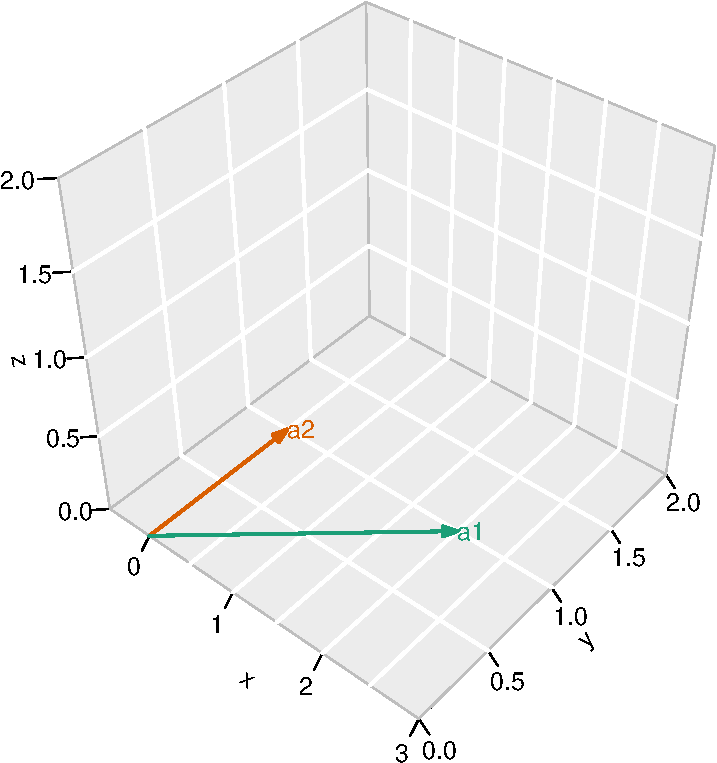
\includegraphics[width=0.5\linewidth]{math4ml_files/figure-beamer/unnamed-chunk-8-1} \end{center}

\end{frame}

\begin{frame}{}
\protect\hypertarget{section-3}{}

\begin{itemize}
\item
  \textbf{linear independence}: \(\{\vv{a}_1, \ldots, \vv{a}_n\}\) are
  linear independent if there exist no \(\lambda_1, \ldots, \lambda_n\)
  (except all being 0) such that
  \[\lambda_1\cdot \vv{a}_1 + \lambda_2 \cdot \vv{a}_2+\ldots + \lambda_n\vv{a}_n=\vv{0}\]

  \begin{itemize}
  \tightlist
  \item
    how about \(\{[2,3]^T, [4,6]^T\}\) ?
  \item
    are \(\{[1,0]^T, [0,1]^T\}\) LI?
  \item
    essentially a way to tell whether there is any \emph{redundant}
    vectors in the set
  \end{itemize}
\item
  \textbf{rank} of \(\vv{A} = [\vv{a}_1, \ldots, \vv{a}_n]\): the
  maximum number of linearly independent column vectors

  \begin{itemize}
  \tightlist
  \item
    the span of the column vectors is called \emph{column space}
  \item
    \emph{rank} also called the \emph{dimension} of the column space
  \item
    \emph{dimension}: the minimum \(\#\) of the vectors needed to span a
    space

    \begin{itemize}
    \tightlist
    \item
      what is the \emph{dimension} for \(R^3\)?
    \end{itemize}
  \end{itemize}
\end{itemize}

\end{frame}

\begin{frame}{Example}
\protect\hypertarget{example-2}{}

The column vectors of the matrix

\[[\vv{a}_1, \vv{a}_2, \vv{a}_3]= \begin{bmatrix} 2 &0 & 1 \\
1&1& 1 \\
0 &0&0
\end{bmatrix}\]

are not linearly independent, as
\[\lambda_1 \vv{a}_1 +\lambda_2\vv{a}_2+\lambda_3\vv{a}_3 = \vv{0}\]

holds for \(\lambda_1=\lambda_2=1, \lambda_3=-2\). In other words, one
of them is redundant. And \(\text{rank}(\vv{A}) = 2\)

\end{frame}

\begin{frame}{Matrix vector multiplication}
\protect\hypertarget{matrix-vector-multiplication}{}

\setbeamercovered{invisible}

\[\vv{A}\vv{x} = \begin{bmatrix}
\vert & \vert &  & \vert\\
\vv{a}_1 & \vv{a}_2 & \ldots & \vv{a}_{n} \\
\vert & \vert & & \vert 
\end{bmatrix} \begin{bmatrix}
x_{1}\\
x_{2}  \\
\vdots  \\
x_{n} 
\end{bmatrix} =  x_1 \begin{bmatrix}
\vert \\
\vv{a}_{1}  \\
\vert 
\end{bmatrix} + x_2 \begin{bmatrix}
\vert \\
\vv{a}_{2}  \\
\vert 
\end{bmatrix}+\ldots + x_n \begin{bmatrix}
\vert \\
\vv{a}_{n}  \\
\vert 
\end{bmatrix}\]

\begin{itemize}
\tightlist
\item
  another view of the multiplication
\item
  \emph{linear combination} of the column vectors of \(\vv{A}\)

  \begin{itemize}
  \tightlist
  \item
    \(x_1\cdot \vv{a}_1 + x_2 \cdot \vv{a}_2+\ldots + x_n\vv{a}_n\)
  \item
    \(\vv{a}_{i}\) are the column vectors and \(x\) are the scalars
  \end{itemize}
\item
  so \ldots{} \(\vv{Ax} = \vv{y}\) essentially solves for what ? \pause 

  \begin{itemize}
  \tightlist
  \item
    \(\vv{y}\) is in the column space of \(\vv{A}\) or not \ldots{}
  \item
    if not, then there is no solution
  \item
    if yes, there will be some solution(s)? unique solution or ?
  \end{itemize}
\end{itemize}

\end{frame}

\begin{frame}{Matrix vector multiplication (some interpretations)}
\protect\hypertarget{matrix-vector-multiplication-some-interpretations}{}

So \(\vv{A}\vv{x}\) is a linear transformation: \(R^n\rightarrow R^m\)

\begin{itemize}
\tightlist
\item
  rotation: rotate \(\vv{x}\) anti-clockwise by \(\theta\)
  \[R\vv{x} = \begin{bmatrix} cos\theta & -sin\theta \\
  sin\theta & cos\theta\end{bmatrix} \begin{bmatrix} x_1\\ x_2\end{bmatrix} = \begin{bmatrix}0.71&-0.71 \\0.71&0.71 \\\end{bmatrix} \begin{bmatrix} x_1\\ x_2\end{bmatrix}\]
  say \(\theta = \pi/4\)
\end{itemize}

\begin{center}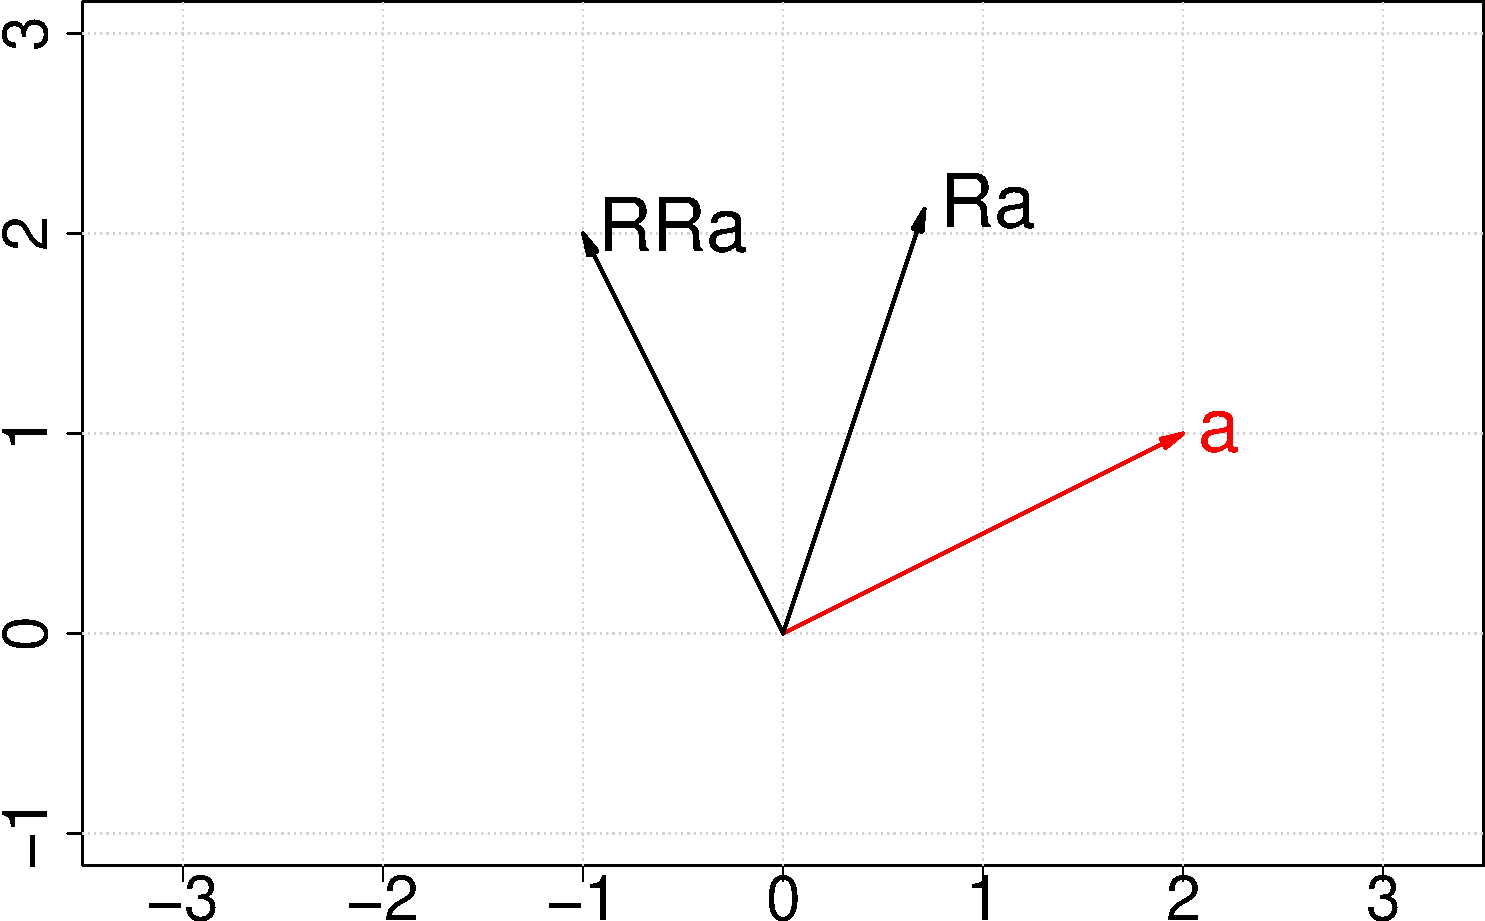
\includegraphics[width=0.5\linewidth]{math4ml_files/figure-beamer/unnamed-chunk-10-1} \end{center}

\end{frame}

\begin{frame}{}
\protect\hypertarget{section-4}{}

\begin{itemize}
\tightlist
\item
  \(\vv{R}\) is a rotation (orthogonal) matrix if
  \(\vv{R}^T = \vv{R}^{-1}\) (what does it imply?)
\item
  \(\vv{R}^T\vv{R} = \vv{R}\vv{R}^T =\vv{I}\) \pause 

  \begin{itemize}
  \tightlist
  \item
    preserves length
    \((\vv{R}\vv{x})^T(\vv{R}\vv{x}) = \vv{x}^T\vv{R}^T\vv{R}\vv{x} = \vv{x}^T\vv{x}\)
  \end{itemize}
\item
  rotation transform is alwasy invertible: inverse means rotating back!
\item
  mathematics is always so reasonable :-)
\end{itemize}

\end{frame}

\begin{frame}{}
\protect\hypertarget{section-5}{}

Projection: project \(\vv{x}\in R^n\) to \(\vv{a}\in R^n\)
\begin{align*}P(\vv{x}, \vv{a}) &= \|\vv{x}\|cos \theta * \frac{\vv{a}}{\|\vv{a}\|} =  \frac{\vv{a}^T\vv{x}}{\vv{a}^T\vv{a}}  \vv{a} \\
&= \frac{\vv{a}\cdot \vv{a}^T\vv{x}}{\vv{a}^T\vv{a}} = \frac{\vv{a}\vv{a}^T}{\vv{a}^{T}\vv{a}}\vv{x}=\vv{Px}\end{align*}

\[\vv{P} = \frac{\vv{a}\vv{a}^T}{\vv{a}^{T}\vv{a}}\]

\begin{itemize}
\tightlist
\item
  \(\vv{P}\) is \(n\) by \(n\) square matrix
\item
  \(\vv{P}\) is a projection matrix: \(\vv{Px}\) returns the projection
\item
  what if we project it again (and again \ldots{}) ?
  \(\vv{P}\ldots\vv{P}\vv{P}\vv{x}\) \pause 

  \begin{itemize}
  \tightlist
  \item
    it remains unchanged,
    \(\vv{P}\ldots\vv{P}\vv{P}\vv{x} = \vv{P}\vv{x}\)
  \item
    or \(\vv{P}\vv{P} = \vv{P}\)
    \[\frac{\vv{a}\vv{a}^T}{\vv{a}^{T}\vv{a}}\frac{\vv{a}\vv{a}^T}{\vv{a}^{T}\vv{a}}= \frac{\vv{aa}^T\vv{aa}^T}{(\vv{a}^T\vv{a})^2}= \frac{\vv{a}\vv{a}^T}{\vv{a}^{T}\vv{a}}\]
  \end{itemize}
\item
  some projection cannot be reversed: some \(\vv{P}\) is not invertible
  !
\item
  mathematics always makes sense :-)
\end{itemize}

\section{Calculus}
\only<article>{Our revision on calculus will be brief. We will only review the concept of partial derivative, gradient, and hessian matrix. You should try to convince yourself all the results listed here if you can.}

\end{frame}

\begin{frame}{Calculus}
\protect\hypertarget{calculus}{}

\begin{itemize}
\item
  univariate derivative \bigskip
\item
  partial derivative \bigskip
\item
  gradient
\end{itemize}

\bigskip

\begin{itemize}
\tightlist
\item
  hessian matrix
\end{itemize}

\bigskip

\begin{itemize}
\tightlist
\item
  quadratic form and its derivative
\end{itemize}

\bigskip

\begin{itemize}
\tightlist
\item
  Lagrange multiplier
\end{itemize}

\end{frame}

\begin{frame}{Derivative}
\protect\hypertarget{derivative}{}

Given function \(f(x): R\rightarrow R\), the derivative is defined as

\[\frac{df}{dx} \equiv Df(x) \equiv \lim_{\Delta x \rightarrow 0} \frac{f(x+\Delta x) - f(x)}{\Delta x} \]

\begin{itemize}
\tightlist
\item
  the growth rate at or near \(x\)
\item
  the derivative points in the direction of steepest ascent of f
\item
  when \(Df(x) =0\), \(f\) doesn't grow or decline near \(x\), or
  \emph{stationary}

  \begin{itemize}
  \tightlist
  \item
    either maximum (negative second derivative) or minimum (positive
    second derivative)
  \item
    saddle point
  \item
    for optimisation, just find \(Df(x) = 0\)
  \end{itemize}
\end{itemize}

\end{frame}

\begin{frame}{Example}
\protect\hypertarget{example-3}{}

\(f(x) = -x^2\) what are the derivatives at -2 and 2?

\begin{itemize}
\tightlist
\item
  \(Df(x) = -2x\);
\item
  at \(x=-2\), \(Df(-2)=4 >0\) points to the right (ascent direction)
\item
  at \(x=2\), \(Df(2) =-4 <0\) points to the left (ascent direction)
\item
  at \(x=0\), \(Df(0) = 0\), it's maximum as \(D^2f(0) =-2<0\) \bigskip
\end{itemize}

\begin{center}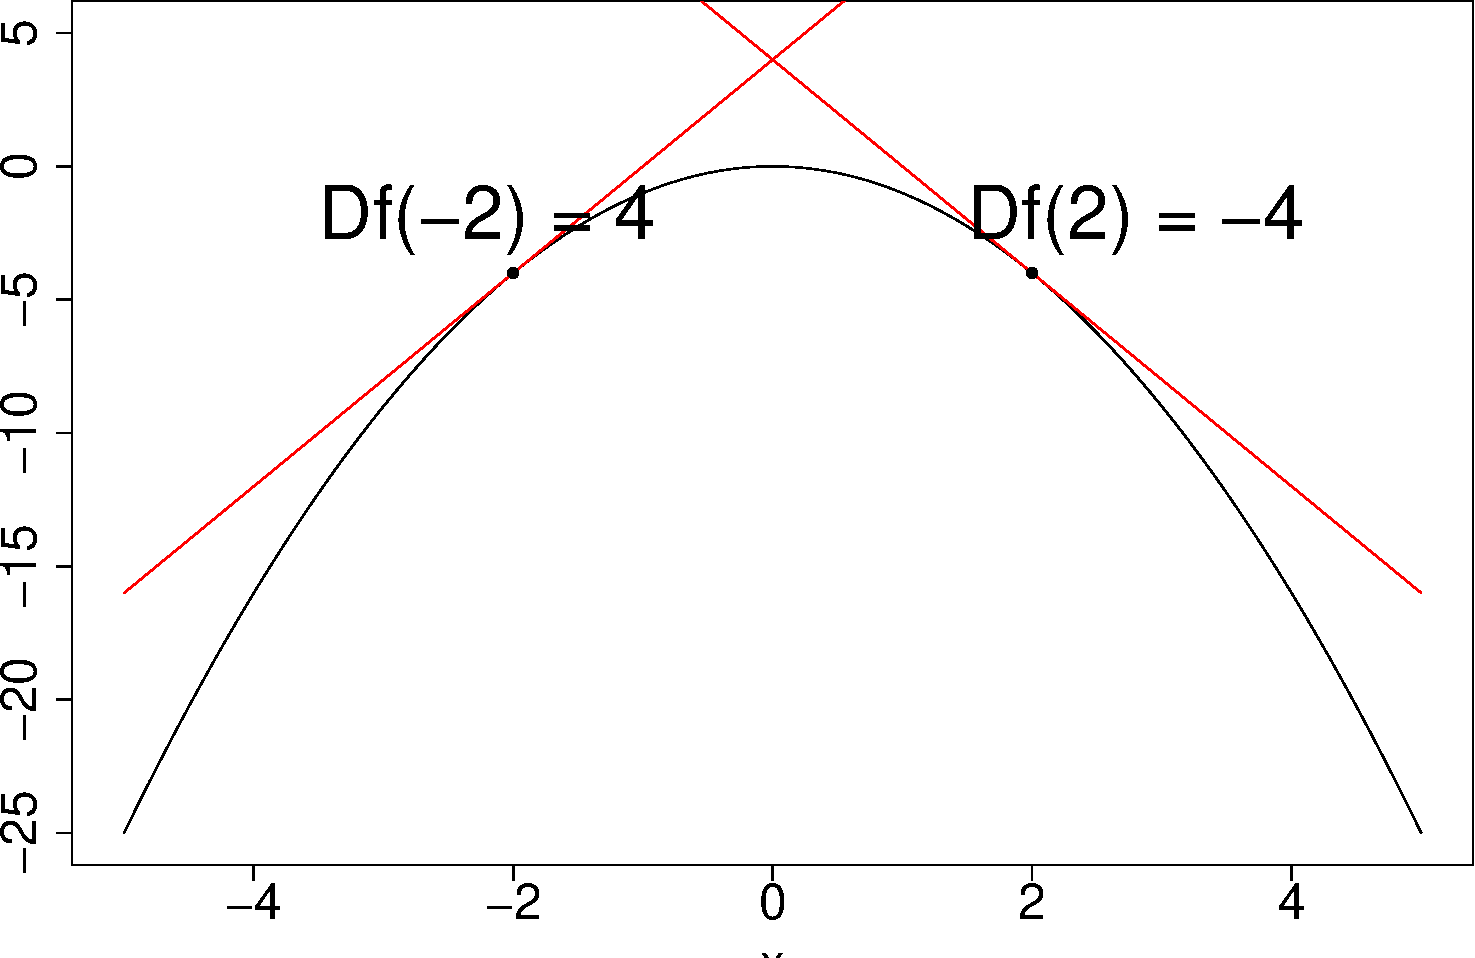
\includegraphics[width=0.6\linewidth]{math4ml_files/figure-beamer/unnamed-chunk-11-1} \end{center}

\end{frame}

\begin{frame}{Partial derivative and gradient}
\protect\hypertarget{partial-derivative-and-gradient}{}

Given function \(f(\vv{x}): R^n\rightarrow R\), partial derivative
w.r.t. \(x_i\) is

\[\frac{\partial f}{\partial x_i} = \lim_{h \rightarrow 0} \frac{f(x_1, \ldots, x_i+h, \ldots, x_n) - f(x_1, \ldots, x_i, \ldots, x_n)}{h} \]

The vector

\[\nabla_{\vv{x}}f=\text{grad} f = \frac{df}{d\vv{x}} = \left [\frac{\partial f(\vv{x})}{\partial x_1}, \frac{f(\vv{x})}{\partial x_2}, \ldots, \frac{f(\vv{x})}{\partial x_n}\right ]\]

\begin{itemize}
\tightlist
\item
  partial derivative measure the growth rate at axis aligned directions
\item
  similarly, the gradient points to the greatest ascent direction
\end{itemize}

\end{frame}

\begin{frame}{Example}
\protect\hypertarget{example-4}{}

Find the gradient of \(f(\vv{x}) = f(x_1, x_2) = x_1^2 +x_2^2\)

\[\nabla_{\vv{x}}f = \left [\frac{\partial f}{\partial x_1}, \frac{\partial f}{\partial x_2}\right ] = [2x_1, 2x_2]\]

\begin{itemize}
\tightlist
\item
  gradient is a vector field: at any input point \([x_1, x_2]\), it
  gives a direction vector \([2x_1, 2x_2]\)
\end{itemize}

\begin{center}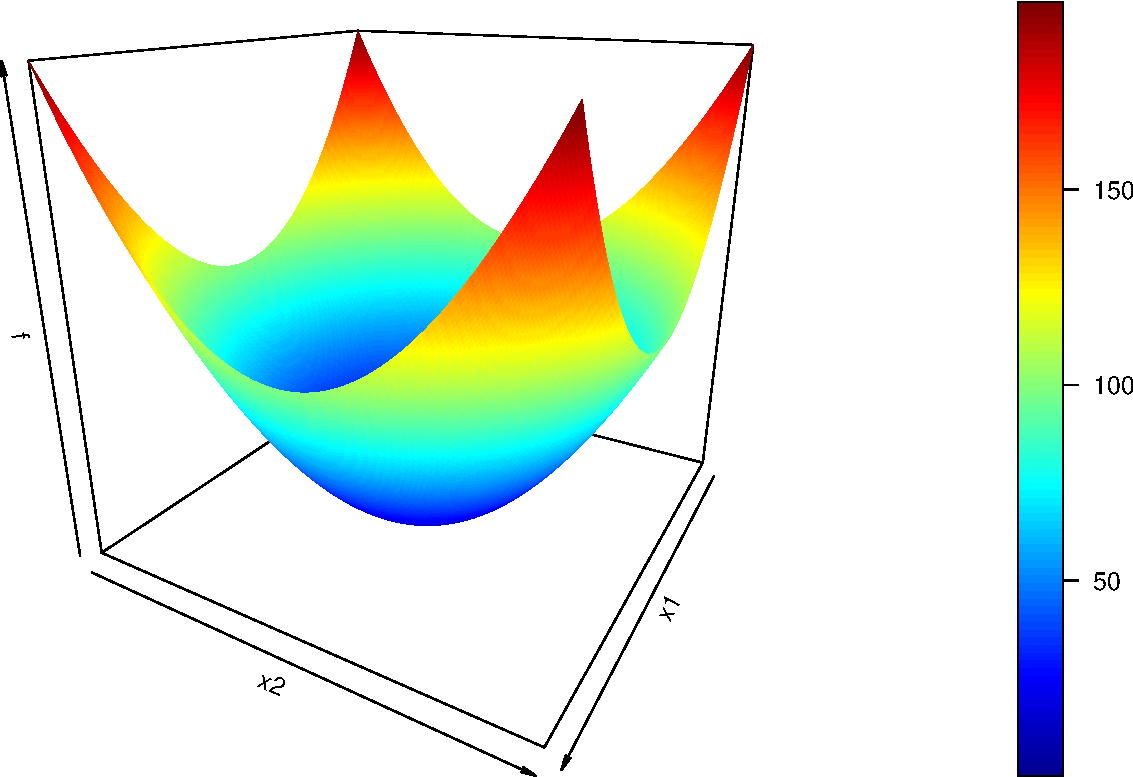
\includegraphics[width=0.6\linewidth]{math4ml_files/figure-beamer/unnamed-chunk-12-1} \end{center}

\end{frame}

\begin{frame}{}
\protect\hypertarget{section-6}{}

\begin{itemize}
\tightlist
\item
  at \(\vv{x} = [1,1]\), the gradient vector is \([2,2]\), pointing to
  steepest ascent direction
\item
  at \(\vv{x} = [1,0]\), the gradient vector is \([2,0]\)
\item
  at \(\vv{x} = [0,0]\), the gradient vanishes
\end{itemize}

\begin{figure}
    \centering
    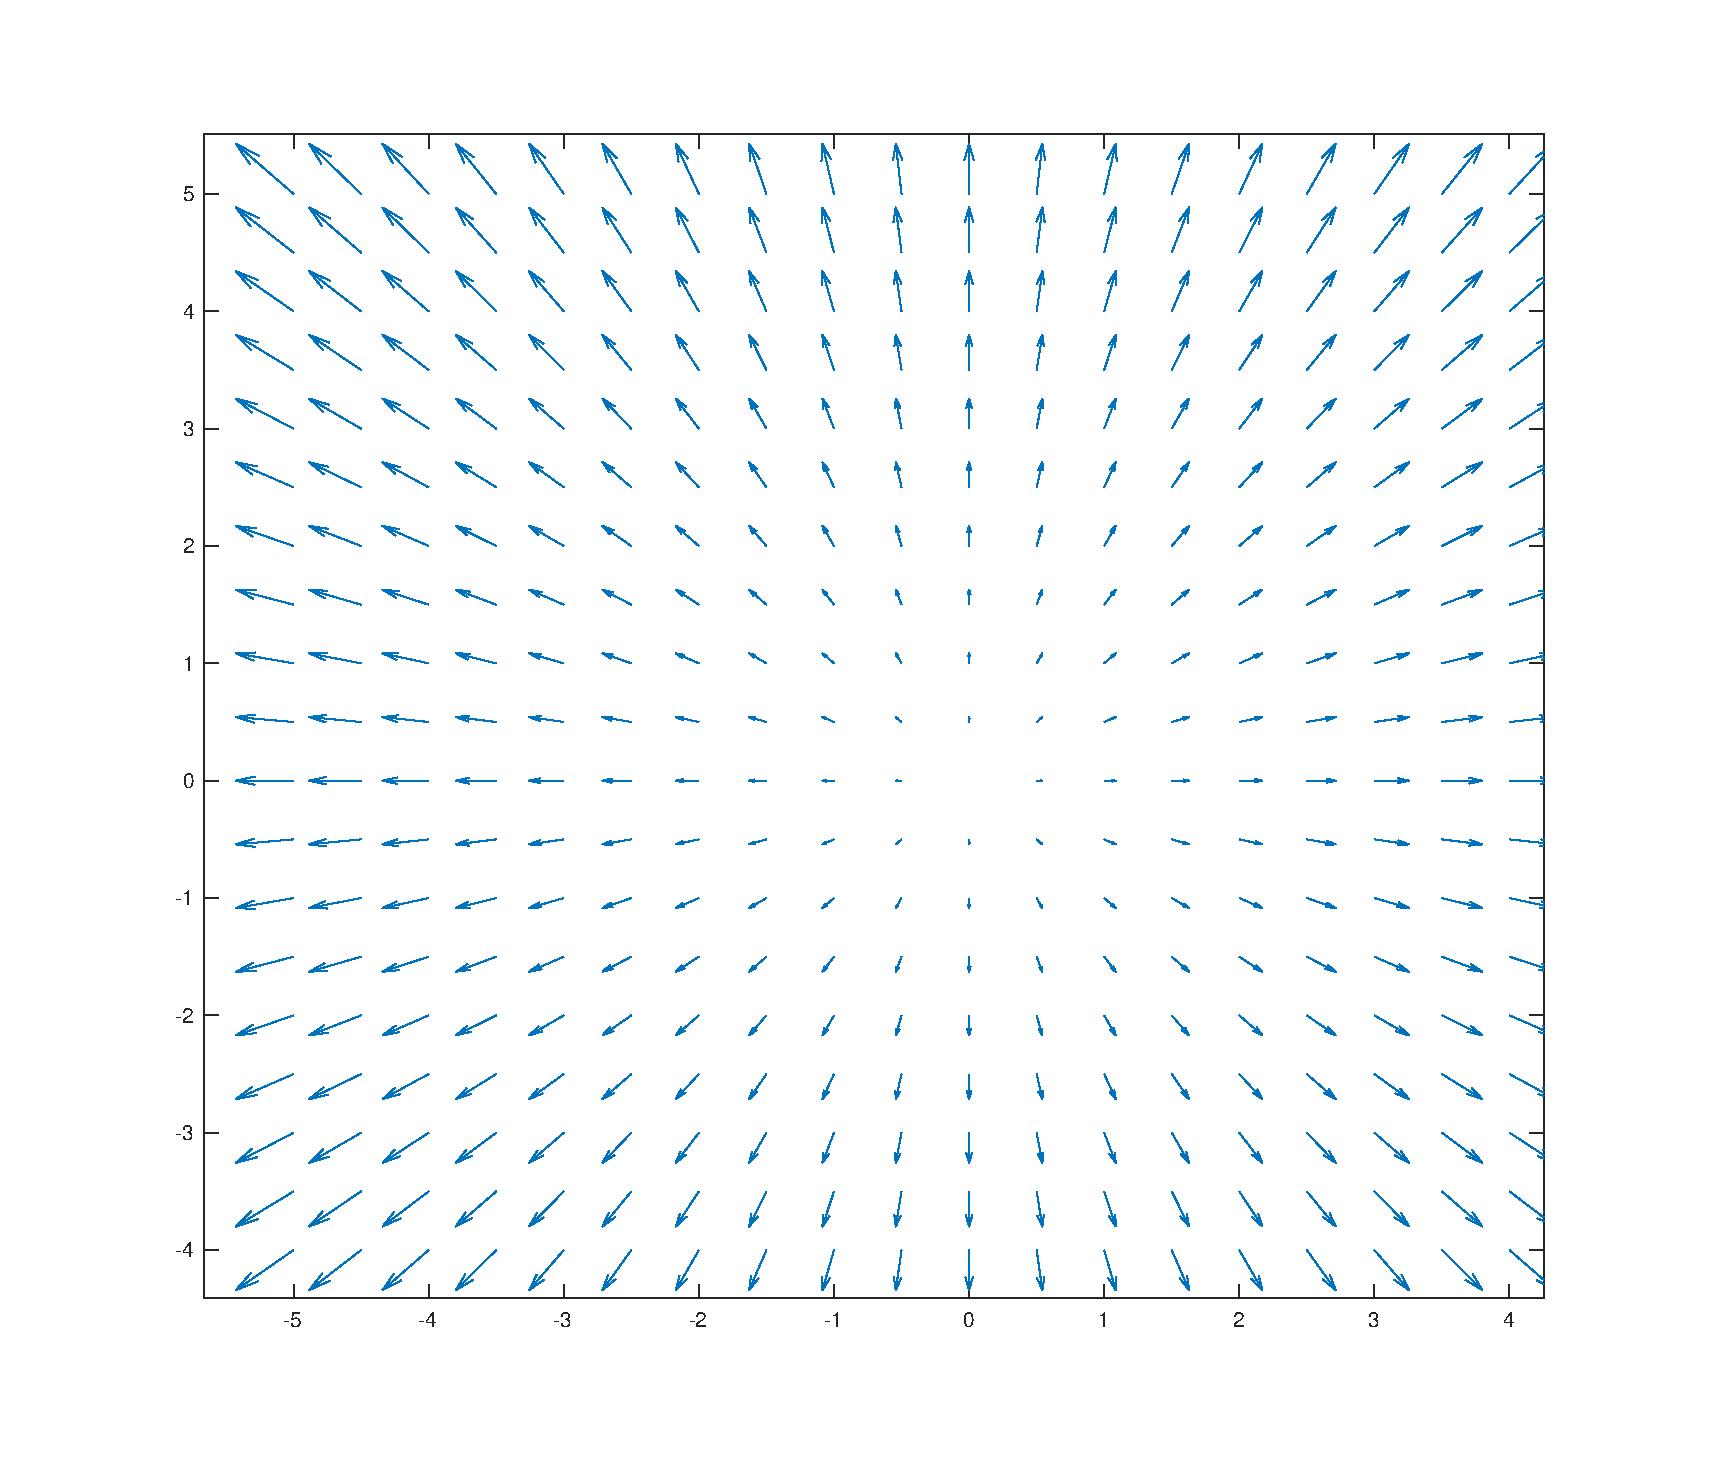
\includegraphics[width = 0.6\textwidth]{./gradvecfield.eps}
 % \caption{Awesome figure}
\end{figure}

\end{frame}

\begin{frame}{Quadratic form \(x^TAx\)}
\protect\hypertarget{quadratic-form-xtax}{}

Another view: \(f(\vv{x}) = x_1^2 +x_2^2= \vv{x}^T \vv{A} \vv{x}\),
where \(\vv{A}\) is \(\vv{I}\) (\emph{verify this!})

\begin{itemize}
\tightlist
\item
  \(\vv{x}^T\vv{Ax}\) is called quadratic form
\item
  generalisation of quadratic function \(f(x) = ax^2 = xax\)
\item
  the gradient is \(\nabla_{\vv{x}} f = 2(\vv{A}\vv{x})^T\) (when \(A\)
  is symmetric)
\item
  the hessian matrix is \(\nabla_{\vv{x}}^2 f = 2\vv{A}\)

  \begin{itemize}
  \tightlist
  \item
    \(f\) has a maximum if \(\vv{A}\) is negative definite (\(a\) is
    negative)
  \item
    \(f\) has a minimum if \(\vv{A}\) is positive definite (\(a\) is
    positive)
  \end{itemize}
\item
  positive definite (P.D.) matrix \(\vv{A}\): \(\vv{x}^T\vv{Ax} >0\) for
  all \(\vv{x}\in R^m\)

  \begin{itemize}
  \tightlist
  \item
    \(\vv{I}\) is P.D., why ?
  \item
    \(f\) has a minimum
  \end{itemize}
\item
  negative definite (N.D.) matrix \(\vv{A}\): \(\vv{x}^T\vv{Ax} <0\) for
  all \(\vv{x}\in R^m\)
\end{itemize}

\end{frame}

\begin{frame}{Example: connecting the dots}
\protect\hypertarget{example-connecting-the-dots}{}

\emph{Given a bunch of numbers \(\vv{x} = [3, 4, 3.5, 5, 6, 5.5]\), to
summarise the data set, sample mean
\[\mu(\vv{x}) = \frac{1}{N} \sum_{i=1}^N {x_i}\] is often used; why ? }

\end{frame}

\begin{frame}{}
\protect\hypertarget{section-7}{}

\begin{itemize}
\tightlist
\item
  \((\mu -x_i)^2\) meansures the distance between \(x_i\) and \(\mu\)
\item
  \(\sum_{i=1}^{N} (\mu -x_i)^2\) measures the total distance or cost
\item
  note that
  \(\mu\begin{bmatrix}1\\ \vdots \\1 \end{bmatrix} - \begin{bmatrix}x_1 \\\vdots \\x_n\end{bmatrix} = \begin{bmatrix}\mu-x_1 \\\vdots \\\mu-x_n\end{bmatrix} \equiv \vv{e}\)
  \begin{align*} 
  \text{Let } f(\mu) &= \sum_{i=1}^{N} (\mu -x_i)^2 = (\mu \vv{1}- \vv{x})^{T}(\mu \vv{1}- \vv{x})= \vv{e}^T\vv{e} = \vv{e}^T\vv{I}\vv{e} \\
  \frac{df}{d\mu} &=  \underbrace{\frac{\partial f}{\partial \vv{e}}\frac{d\vv{e}}{d\mu}}_{\text{chain rule}}= 2\vv{e}^T\vv{1} = 2(\mu\vv{1} - \vv{x})^T \vv{1}
  \end{align*}
\end{itemize}

\bigskip

set the derivative to 0 \begin{align*} 
\mu\vv{1}^T\vv{1} -\vv{x}^T \vv{1}= 0 \Rightarrow  \mu = \frac{\vv{1}^T\vv{x}}{\vv{1}^T\vv{1}} = \frac{\sum_{i}^N x_i}{N}
\end{align*}

\begin{itemize}
\tightlist
\item
  can you tell it is actually a projection ?
\end{itemize}

\end{frame}

\begin{frame}{}
\protect\hypertarget{section-8}{}

\begin{itemize}
\item
  note that the projection of \(\vv{x}\) on \(\vv{1}\) is
  \[P(\vv{x}, \vv{1}) = \frac{\vv{1}^T\vv{x}}{\vv{1}^T\vv{1}} \vv{1} = \mu \vv{1}\]
\item
  this is a ML model actually (specific case)
\item
  for this simple example, we have used

  \begin{itemize}
  \tightlist
  \item
    linear algebra
  \item
    vector calculus
  \end{itemize}
\item
  how about probability theory ?
\end{itemize}

\end{frame}

\hypertarget{probability-theory}{%
\section{Probability theory}\label{probability-theory}}

\begin{frame}{Probability theory}
\protect\hypertarget{probability-theory-1}{}

\begin{itemize}
\tightlist
\item
  Random variable \bigskip
\item
  Probability distribution \bigskip
\item
  Probability mass function and density function \bigskip
\item
  Probability rules \bigskip
\item
  Expectation, variance, covariance \bigskip
\item
  Conditional expectation
\end{itemize}

\end{frame}

\begin{frame}{Random variable and probability distribution}
\protect\hypertarget{random-variable-and-probability-distribution}{}

\textbf{Random variable} \(X\) associates with a \textbf{probability
distribution} \(P(X)\)

\begin{itemize}
\tightlist
\item
  formally, a r.v. is a mapping from sample space \(\Omega\) to a target
  space \(\mathcal{T}\)
\item
  e.g.~toss a fair coin twice, r.v. \(X\) is the number of heads turned
  up

  \begin{itemize}
  \tightlist
  \item
    the sample space is \(\Omega =\{HH, TT, HT, TH\}\)
  \item
    target space is \(T =\{0,1,2\}\)
  \item
    the probability distribution is \[P(X) = \begin{cases} 0.25 & X=0 \\
    0.5 & X=1 \\
    0.25 & X=2 \end{cases}\]
  \end{itemize}
\item
  the distribution \(P\) must satisfy
  \[P(X=x) >0, \text{ and } \sum_{x\in T} P(X=x) =1\]
\end{itemize}

\end{frame}

\begin{frame}{Random variable - discrete r.v.}
\protect\hypertarget{random-variable---discrete-r.v.}{}

If r.v. \(X\)'s target space \(\mathcal{T}\) is discrete

\begin{itemize}
\tightlist
\item
  \(X\) is called \textbf{discrete random variable}
\item
  the probability distribution \(P\) is called \textbf{probability mass
  function} (p.m.f.)
\item
  and \[0\leq P(X=x) \leq 1, \text{ and } \sum_{x\in T} P(X=x) =1\]
\end{itemize}

\end{frame}

\begin{frame}{Example - discrete r.v.}
\protect\hypertarget{example---discrete-r.v.}{}

\textbf{Bernoulli distribution} Tossing a coin ,
\(\mathcal{T} = {1, 0}\) (1 is \(H\), 0 is \(T\)),
\[P(X=1) = p , P(X=0) = 1-p, 0\leq p\leq 1\]

\textbf{Binomial distribution} Tossing a coin \(N\) times, the r.v.
\(X\) is the number of head shows up
\[P(X=k) = \binom{N}{k} \cdot p^k(1-p)^{N-k}\]

\begin{itemize}
\item
  what's the relationship between Binomial and Bernoulli?

  \bigskip
\end{itemize}

\textbf{Multinoulli distribution} Throw a fair 6-facet die,
\(\mathcal{T} = {1, 2,\ldots, 6}\), the distribution is \[P(X=i) = 1/6\]

\emph{Verify the above \(P\)s satisfy the conditions of p.m.f.}

\end{frame}

\begin{frame}{Random variable - continuous r.v.}
\protect\hypertarget{random-variable---continuous-r.v.}{}

If r.v. \(X\)'s target space \(\mathcal{T}\) is continuous

\begin{itemize}
\tightlist
\item
  \(X\) is called \textbf{continuous random variable }
\item
  the probability distribution \(p\) is called \textbf{probability
  density function} (p.d.f.)
\item
  and satisfies \[p(x) \geq 0, \text{ and } \int_{x\in T} p(x) dx = 1\]
\item
  pdf is not probability as \(p(x)\) can be greater 1;
\item
  for \(\forall x\) \(P(X=x) =0\)\\
\item
  calculate probability over an interval: e.g.
  \[P(X \in [a,b]) = \int_{a}^b p(x) dx\]
\end{itemize}

\end{frame}

\begin{frame}{Example - continuous r.v.}
\protect\hypertarget{example---continuous-r.v.}{}

\textbf{Uniform distribution} \(\mathcal{T} = [0,1]\), \(X\) has equal
chance to take any value between 0 and 1; the pdf is
\[p(x) = \begin{cases} 1 & x\in [0,1] \\
0 & \text{otherwise} \end{cases} \]

\begin{center}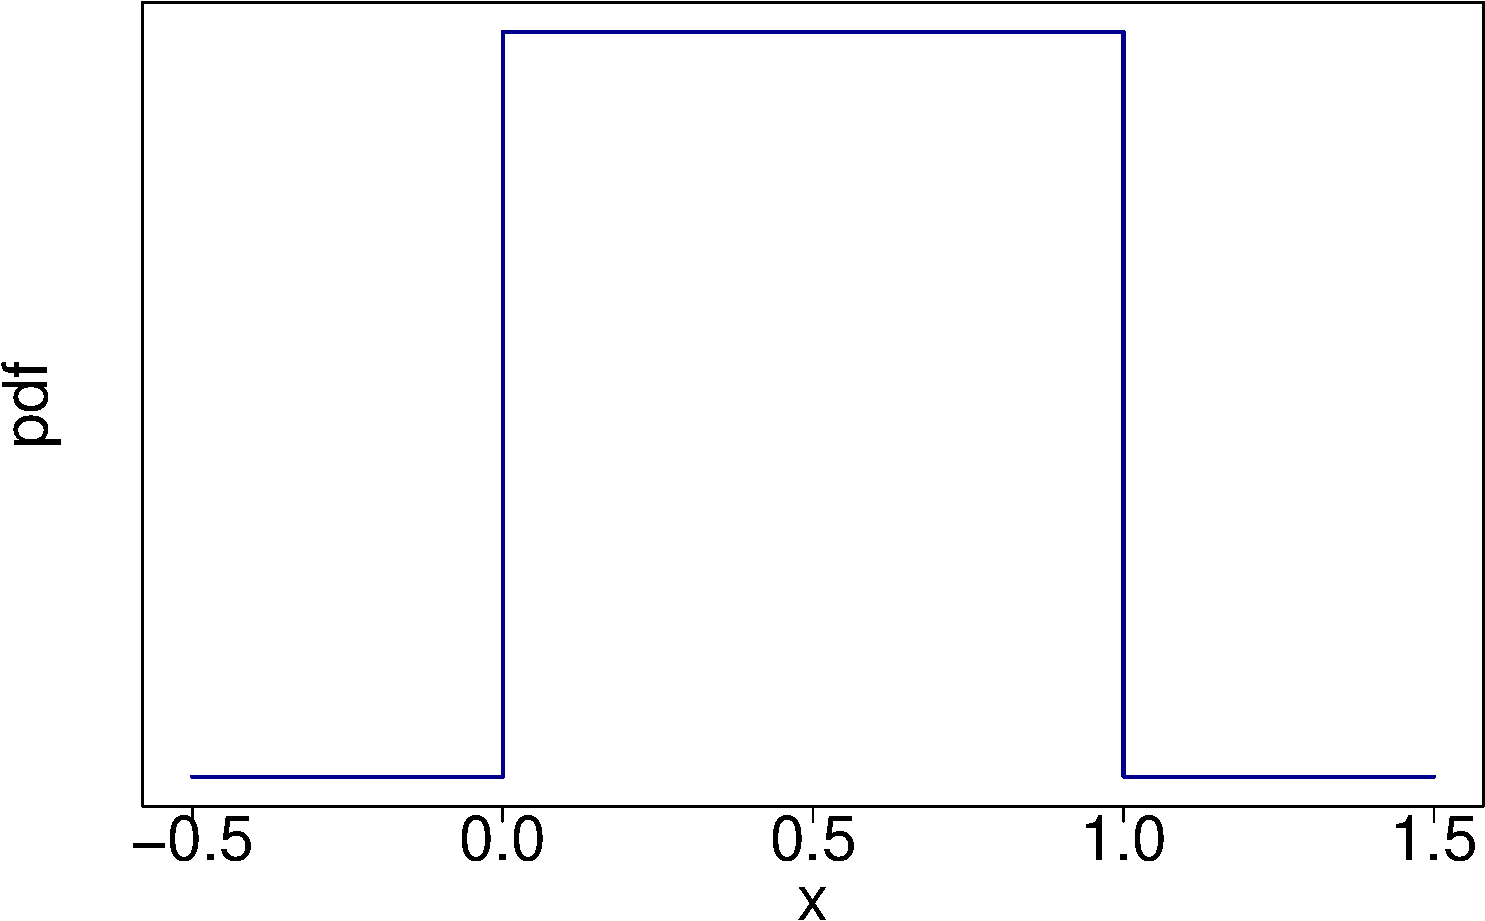
\includegraphics[width=0.5\linewidth]{math4ml_files/figure-beamer/unnamed-chunk-14-1} \end{center}

Easy to verify \(\int_0^1 p(x)dx = \int_0^1 dx =1\) \bigskip

What's the probability that \(0<X<0.5\) ?

\end{frame}

\begin{frame}{Example - continuous r.v.}
\protect\hypertarget{example---continuous-r.v.-1}{}

\textbf{Gaussian distribution} \(\mathcal{T} = R\), or \(X \in R\) the
pdf is

\[p(x) = \normal{x; \mu}{\sigma^2}=\frac{1}{\sigma \sqrt{2\pi}} e^{-\frac{1}{2}(\frac{x-\mu}{\sigma})^2}\]
\((\frac{x-\mu}{\sigma})^2\) is a distance measure: how far \(x\) is
away from \(\mu\) (measured by \(\sigma\) as a unit)

\begin{center}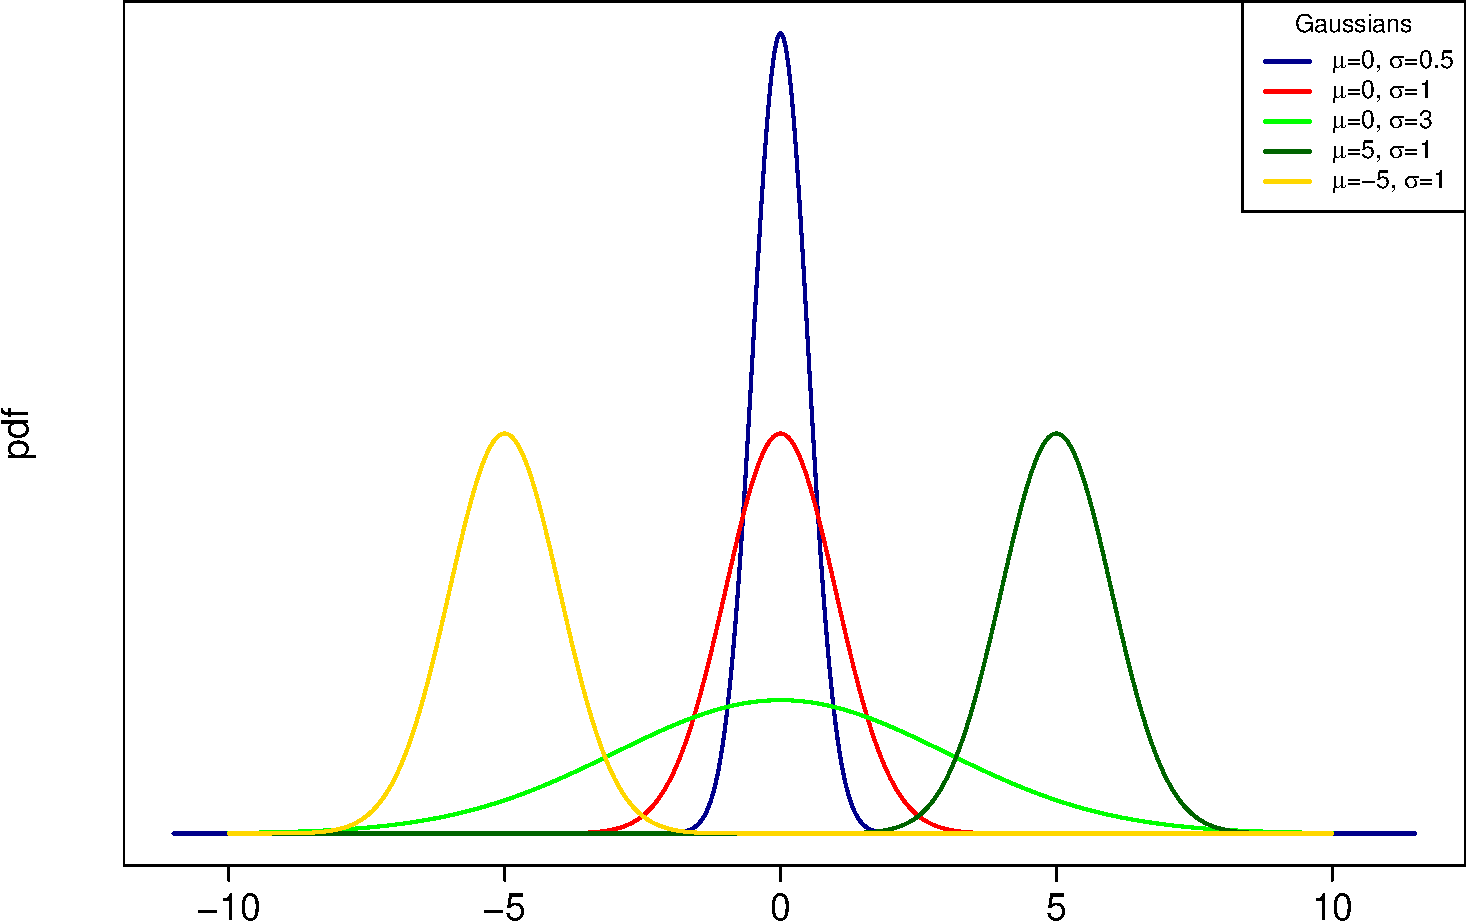
\includegraphics[width=0.65\linewidth]{math4ml_files/figure-beamer/unnamed-chunk-15-1} \end{center}

\end{frame}

\begin{frame}{Question}
\protect\hypertarget{question}{}

Calculate quickly: \[\int_{-\infty}^{\infty} e^{-\frac{1}{2}x^2}dx = ?\]

\bigskip

For \(X\sim \normal{\mu}{\sigma}\), what is \(P(X<\mu)=\)?

\end{frame}

\begin{frame}{Joint distribution}
\protect\hypertarget{joint-distribution}{}

\begin{itemize}
\tightlist
\item
  r.v. \(\vv{X} = [X_1, X_2, \ldots, X_n]^T\) can be multidimensional
  (each \(X_i\) is r.v.)

  \begin{itemize}
  \tightlist
  \item
    essentially a \emph{random vector}
  \end{itemize}

  \bigskip
\item
  Still satisfies the same requirements
  \[\forall \vv{x}, 0<P(\vv{X}=\vv{x}) <1,\; \sum_{x_1}\sum_{x_2}\ldots\sum_{x_n} P(\vv{X} =[x_1, x_2, \ldots, x_n]) =1\]
  or
  \[\forall \vv{x}, p(\vv{X}=\vv{x}) >0,\; \int\int\ldots\int p(\vv{X} =\vv{x})d{x_1}d{x_2\ldots dx_{n}} =1\]
  \bigskip 
\item
  for bivariate case, i.e. \(n=2\), \(X_1, X_2\) are
  \textbf{independent} if \(P(\vv{X}) = P(X_1)P(X_2)\) (e.g.~rolling two
  dice independently)
\end{itemize}

\end{frame}

\begin{frame}{Example: discrete joint distribution}
\protect\hypertarget{example-discrete-joint-distribution}{}

The joint distribution of \(X\) snow or not, \(Y\in\) \{\text{spring},
\text{summer}, \text{autumn}, \text{winter}\} represents the season that
\(x\) belongs to : \bigskip 

\begin{table}\centering
\begin{tabular}{ l | c | c | c | c}
   \centering                    
   & $y=\text{Spring}$ & $y=\text{Summer}$ &$y=\text{Autumn}$ & $y=\text{winter}$\\ 
   \hline
  $x= F$ & 0.05 & 0.25 & 0.075& 0\\
    \hline 
  $x= T$ & 0.2 & 0 & 0.175& 0.25\\ 
\end{tabular}
\end{table}
\bigskip

It is easy to verify that\\
\[\sum_x\sum_y p(x, y) = 1\]

\end{frame}

\begin{frame}{Example: continuous joint distribution}
\protect\hypertarget{example-continuous-joint-distribution}{}

If \(X,Y\)'s joint p.d.f is
\[p(x,y) = \frac{1}{2\pi\sigma_x\sigma_y} e^{-\frac{1}{2}[(\frac{x-\mu_x}{\sigma_x})^2 +(\frac{y-\mu_y}{\sigma_y})^2] }\]

\(X,Y\) are bivariate Gaussian distributed

\bigskip

X,Y are \emph{independent} for this case, why ?

\end{frame}

\begin{frame}{Probability rules}
\protect\hypertarget{probability-rules}{}

There are only two probability rules (integration for continuous r.v.):

\begin{enumerate}
    \item product rule: \[ p(x, y) = p (y|x)p(x) = p(x|y)p(y)\]
    \item sum rule (marginalisation): \[ p (x) = \sum_y p(x, y),\; p(y) = \sum_x p(x, y)\]
\end{enumerate}

\end{frame}

\begin{frame}{Conditional probability}
\protect\hypertarget{conditional-probability}{}

Conditional probability distribution (by product rule):
\[p (x| y) = \frac{p(x, y)}{p(y)}\]

\begin{itemize}
\tightlist
\item
  probability distribution of \(x\) conditional on the value of \(y\)
\end{itemize}

\bigskip

\begin{table}\centering
\begin{tabular}{ l | c | c | c | c}
   \centering                    
   & $y=\text{Spring}$ & $y=\text{Summer}$ &$y=\text{Autumn}$ & $y=\text{winter}$\\ 
   \hline
  $x= F$ & 0.05 & 0.25 & 0.075& 0\\
    \hline 
  $x= T$ & 0.2 & 0 & 0.175& 0.25\\ 
\end{tabular}
\end{table}

\bigskip

\begin{itemize}
\item
  \(P(Y= \text{Spring})\) ? use sum rule
  \(P(Y = \text{Spring}) = \sum_{x=\{T,F\}} P(X=T,Y=\text{Spring}) =0.05+0.2=0.25\)
\item
  \(P(X=T | Y= \text{Spring})\) ?
  \(P(x=T | y = \text{Spring}) = \frac{P(x=T, y=\text{Spring})}{P(y=\text{Spring})}=\frac{0.2}{0.25}=0.8\)
\end{itemize}

\end{frame}

\begin{frame}{Expectation and variance}
\protect\hypertarget{expectation-and-variance}{}

\textbf{Expection} of a r.v. is defined as
\[\E{g(X)} = \sum_x g(x) P(x) \text{ or } \E{g(X)} = \int g(x) P(x)dx\]

\begin{itemize}
\tightlist
\item
  \(\E{a} = a\), \(a\) is a constant (not r.v.)
\item
  \(\E{\E{X}} = \E{X}\)
\item
  \(\E{aX +bY} = a\E{X} + b\E{Y}\): linearity
\end{itemize}

\bigskip

\textbf{Variance} of a r.v. is defined as
\[\Var{g(X)} = \E{(g(X)-\E{g(X)})^2}\]

\begin{itemize}
\tightlist
\item
  \(\Var{X} = \E{X^2} - \E{X}^2\)
\item
  \(\Var{aX} = a^2\Var{X}\)
\end{itemize}

\bigskip

\emph{Prove them or convince yourself !}
\only<article>{A very useful identity that links expectation and variance together is 
\[\Var{x} = \E{x^2} - \E{x}^2 , \] which can be proved as follows:
\[ \Var{x} = \E{x^2 -2\E{x} x + \E{x}^2} = \E{x^2} -2\E{x}^2 + \E{x}^2 = \E{x^2} - \E{x}^2; \]
 the second equality holds because $\E{x}=\mu$  is a constant. Note that $\E{x^2}$ is called the \textit{second moment} of r.v. $x$.}

\end{frame}

\begin{frame}{Example}
\protect\hypertarget{example-5}{}

\(X\) is a Bernoulli r.v. with parameter \(p=0.5\); what is \(\E{X}\)?

\begin{itemize}
\tightlist
\item
  \(\E{X} = 1\times P(X=1) + 0\times P(X=0) = p =0.5\);
\end{itemize}

\bigskip

\(Y\) is a Binomial r.v. with \(N=10, p=0.5\), what is \(\E{Y}\)?

\begin{itemize}
\tightlist
\item
  \(Y= \sum_{i=1}^{N} X = N\times X\)
\item
  \(\E{Y} = \E{N\times X} = N\times \E{X} = N\times p = 5\)
\item
  interpretation: you expect to see 5 successes out of 10 (on average
  the result is 5 if you repeat the experiment a lot of times)
\end{itemize}

\end{frame}

\begin{frame}{General advice on reading maths}
\protect\hypertarget{general-advice-on-reading-maths}{}

\begin{tcolorbox}[colback=red!5!white]
  {\large ``The fish trap exists because of the fish. Once you've gotten the fish you can forget the trap. The rabbit snare exists because of the rabbit. Once you've gotten the rabbit, you can forget the snare. Words exist because of meaning. Once you've gotten the meaning, you can forget the words. Where can I find a man who has forgotten words so I can talk with him?''}
  \hspace*\fill{\small--- Zhuang Zhou}
\end{tcolorbox}

\begin{itemize}
\tightlist
\item
  maths intuition is more important than equations
\end{itemize}

\bigskip

\begin{itemize}
\tightlist
\item
  think first then verify your beliefs by reading (different) text books
  or code it up and check
\end{itemize}

\bigskip

\begin{itemize}
\tightlist
\item
  stand higher and look at a greater picture

  \begin{itemize}
  \tightlist
  \item
    accepting intermediate results without fully understanding is
    totally cool
  \end{itemize}
\end{itemize}

\end{frame}

\end{document}
